\documentclass[a4paper,12pt,titlepage,hidelinks,final]{article}

% Paquetes
\usepackage[spanish,es-lcroman]{babel}
\usepackage[utf8]{inputenc}
\usepackage{alltt}
\usepackage{verbatim}
\usepackage[cache=false]{minted}
\usepackage{listings}
\usepackage{caption}
\usepackage{titlesec}
\usepackage[hyperfootnotes=false]{hyperref}
\usepackage[nomain,xindy,toc,acronym]{glossaries}
%   - Visual
\usepackage{float}
\usepackage{setspace}
\usepackage{xspace}
\usepackage{xcolor}
\usepackage{graphicx}
\usepackage{amssymb}
\usepackage{amsthm}
\usepackage{tikz}
\usepackage{fontspec}
%   - Índices
\usepackage[xindy]{imakeidx}

\usepackage{appendix}

% Configuración
%   - Espacio entre el texto principal y las notas al pie
\setlength{\skip\footins}{1cm}
%   - Espacio entre notas al pie
\setlength{\footnotesep}{0.5cm}
%   - Formatos
% \setmainfont{Droid serif} % Si se desea cambiar la tipografía
\titleformat{\paragraph}{\normalfont\normalsize\bfseries}{\theparagraph}{1em}{}
\titlespacing*{\paragraph}{0pt}{3.25ex plus 1ex minus .2ex}{1.5ex plus .2ex}
\setlength{\parskip}{0.6em} % Separación entre párrafos
\setlength{\parindent}{2em} % Sangría de cada párrafo
%   - Resaltado de sintaxis
\setminted{
  fontsize=\small,
  style=bw % o style=colorful para blanco y negro
}
%     + Define el ambiente {phpcode} para código PHP
\newminted{php}{linenos,style=colorful}
%     + Define el comando \phpfile{path} para código PHP desde archivos externos
\newmintedfile{php}{linenos,style=colorful}
%     + Define el ambiente {bashcode} para comandos de CLI
\newminted{bash}{breaklines=true}
%     + Define el comando \bashfile{path} para comandos de CLI desde archivos externos
\newmintedfile{bash}{breaklines=true}
%     + Define el ambiente {jsoncode} para código JSON
\newminted{json}{}
%     + Define el comando \jsonfile{path} para código JSON desde archivos externos
\newmintedfile{json}{}
%     + Define el ambiente {httpcode} para sesiones HTTP
\newminted{http}{breaklines=true,breakatwhitespace=false}
%     + Define el comando \httpfile{path} para sesiones HTTP desde archivos externos
\newmintedfile{http}{breaklines=true}
%   - Formato de los glosarios
\setglossarystyle{altlist}
%   - Formato de bloques preformateados
\lstset{
  basicstyle=\small\ttfamily,
  columns=flexible,
  breaklines=true
}
%   - Formato de los \subparagraphs para que tengan un salto de línea que los separe del texto
\titleformat{\subparagraph}{\normalfont\normalsize\bfseries}{\thesubparagraph}{1em}{}
\titlespacing*{\subparagraph}{\parindent}{3.25ex plus 1ex minus .2ex}{.75ex plus .1ex}
%   - Nombre y título para los bloques de código de minted
\renewcommand{\listingscaption}{Bloque de código}
\renewcommand{\listoflistingscaption}{Listado de bloques de código}

\captionsetup{aboveskip=0pt}

% Definición de ambientes
%   - displaycode: para mostrar código
\newenvironment{displaycode}{\begin{alltt}}{\end{alltt}}
%   - code: para mostrar código
%\newenvironment{code}{\color{Sepia}\verbatim}{\endverbatim}
\newenvironment{code}{\verbatim}{\endverbatim}

% Comandos personalizados

% {\fechaPresentacion} :: para escribir la fecha de presentación del trabajo
\newcommand{\fechaPresentacion}{\today}
% {\unlp} :: para escribir "Universidad Nacional de La Plata"
\newcommand{\unlp}{Universidad Nacional de La Plata}
% {\facultad} :: para escribir "Facultad de Informática"
\newcommand{\facultad}{Facultad de Informática}
% {\cespi} :: para escribir "CeSPI"
\newcommand{\cespi}{CeSPI}
% {\direccionDesarrollo} :: Para escribir "Dirección de Desarrollo del CeSPI"
\newcommand{\direccionDesarrollo}{Dirección de Desarrollo del {\cespi}}
% {\tituloTrabajo} :: Para escribir el título de la tesina
\newcommand{\tituloTrabajo}{Propuesta de una solución de Monitoreo para sistemas del {\cespi}.}
% \tituloTrabajoDosLineas :: Para escribir el título de la tesina en dos líneas (carátula)
\newcommand{\tituloTrabajoDosLineas}{Propuesta de una solución de Monitoreo\\* para sistemas del {\cespi}}
% {\fedeotaran} :: para escribir "Federico Otarán"
\newcommand{\fedeotaran}{Federico Otarán}
% {\otaranfede} :: para escribir "Otarán, Federico"
\newcommand{\otaranfede}{Otarán, Federico}
% {\nicaperera} :: para escribir "Nicanor Perera"
\newcommand{\nicaperera}{Nicanor Perera}
% {\otaranfede} :: para escribir "Otarán, Federico"
\newcommand{\pereranica}{Perera, Nicanor}

% \eng{English expression} :: para denotar que "English expression" está en inglés
\newcommand{\eng}[1]{\textit{#1}}

% {\caratula} :: para generar la carátula de la tesina
\newcommand{\caratula}{
  \begin{center}
    
\includegraphics{src/images/caratula/unlp.png}\\
    \huge{\unlp}\\
    \vspace{5mm}
    \huge{\facultad}\\
    \vspace{5mm}
    \large{Tesina de la Licenciatura}\\
    \vspace{15mm}
    \huge{\tituloTrabajoDosLineas}\\
    \vspace{10mm}
    \large{\textbf{\pereranica} \\
    \textbf{\otaranfede}}\\
    \vspace{20mm}
    \large{Director: Luengo, Miguel}\\
    \large{Asesor Profesional: Rodriguez, Christian Adrián}\\
    \vspace{20mm}
    \normalsize{\fechaPresentacion}\\
  \end{center}
}

\addto\captionsspanish{%
  \renewcommand\appendixname{Anexo}
  \renewcommand\appendixpagename{Anexos}
  \renewcommand\appendixtocname{Anexos}
}

\addto\extrasspanish{%
  \def\sectionautorefname{capítulo}%
  \def\subsectionautorefname{sección}%
  \def\subsubsectionautorefname{sección}%
  \renewcommand{\appendixautorefname}{anexo}%
}

% {\checkmark} :: para imprimir un check (tilde)
\def\checkmark{\tikz\fill[scale=0.4](0,.35) -- (.25,0) -- (1,.7) -- (.25,.15) -- cycle;}


% Generación de glosario e índices
\loadglsentries{src/glosario/glosario}
\makeglossaries
\makeindex[name=palabras,title=Indice de palabras]

\begin{document}
  % Carátula
  \thispagestyle{empty} % Oculta numeración de las páginas
  \setcounter{page}{0}
  \caratula
  \newpage

  % Página en blanco
  \newpage

  % Meta previa al contenido principal
  \setcounter{secnumdepth}{0}
  \setcounter{tocdepth}{4}
  \setcounter{page}{1}
  \pagenumbering{Roman}

  %   - Tabla de contenidos
  \begingroup
    \setlength{\parskip}{0pt}   % Sin separación entre párrafos
    \setlength{\parindent}{0pt} % Sin sangría en cada párrafo
    \tableofcontents
  \endgroup
  \newpage

  % Contenido principal
  \pagenumbering{arabic}      % Tipo de numeración de páginas a usar
  %   - Introducción
  \section{Introducción}
\label{intro}

Los desarrolladores de sistemas informáticos de la Dirección de Desarrollo del
\gls{acro:cespi}, \gls{acro:unlp}, construyen aplicaciones para clientes
internos y externos a la \gls{acro:unlp}. En esta oficina se aplican técnicas
\gls{acro:devops} para agilizar el despliegue y mantener en sintonía los
ambientes de desarrollo, testing y producción. Su equipo de trabajo está
integrado por más de una docena de profesionales en informática, los cuales
están a cargo de diferentes proyectos.

Parte importante de la implementación y mantenimiento de estos sistemas es la
recolección y análisis de datos de su funcionamiento. Este análisis es
importante para conocer la salud de los servidores y el rendimiento de los
procesadores, detectar fallas en el hardware y/o software, descubrir
comportamientos que afecten la funcionalidad de las aplicaciones y tomar
decisiones que mejoren la productividad y calidad de los servicios brindados.

Recoger datos y calcular estadísticas sobre servidores, aplicaciones y tráfico
puede aumentar la seguridad en la toma de decisiones y permitir la anticipación
a problemas futuros.

La disciplina de recolectar datos de forma constante a lo largo del tiempo
facilita la comprensión de los eventos que ocurren en cada instante,
permitiendo contrastar un valor actual con valores previos. Esto proporciona la
capacidad de respaldar decisiones con datos reales.

En la actualidad existen una gran variedad de herramientas que pueden ser
usadas para tener un seguimiento de métricas sobre servicios de software, y es
posible integrar estas herramientas para crear un sistema que permita obtener,
almacenar y visualizar los resultados. Hoy en día, no todos los proyectos
dentro del \gls{acro:cespi} cuentan con herramientas adecuadas para esta tarea.


\subsection{Objetivo}
\label{objetivo}

El objetivo que tiene la investigación de esta tesis es plasmar el resultado de
comparar y proponer una estrategia de recolección, análisis y utilización de
información de la infraestructura y las aplicaciones del \gls{acro:cespi}, que
permita simplificar y enriquecer su análisis posterior y resulte en un
monitoreo eficiente.

Se espera que cualquier problema con las aplicaciones pueda ser detectado y
analizado en un contexto global, y que diferentes fuentes de registros de datos
puedan ser correlacionadas para aprender aún más sobre el estado de los
proyectos. Para lograr esto realizará una evaluación el estado de arte de las
estrategias de recolección de datos, estadísticas, monitoreo y generación de
alertas.  A partir de este análisis, habrá que relevar las herramientas que
permitan implementar dichas estrategias, permitiéndo así proceder hacia un
diseño de una infraestructura que las utilice.

Finalmente se integrará el sistema de monitoreo a la infraestructura actual de
forma automatizada mediante prácticas \gls{term:devops}, y buscará sentar las
bases para que se puedan obtener tableros de control que permitan visualizar el
estado de la infraestructura completa y que permita profundizar en resultados
según los criterios de los diferentes perfiles de usuario.

Se busca entonces con este procedimiento identificar los datos de importancia a
ser recolectados para alimentar un sistema de monitoreo que permita alertar de
forma inteligente cuando alguna parte crítica del sistema se vuelva inestable o
no responda a los resultados deseables. A su vez, se quiere conseguir la
disponibilidad en todo momento de una vista de alto nivel del funcionamiento de
toda la infraestructura, que facilite la toma de decisiones en distintos
niveles según los intereses de los usuarios.

Teniendo en cuenta todo lo mencionado hasta ahora, se buscará alcanzar una
solución de monitoreo que permita entender a la infraestructura no como piezas
separadas, sino como un conjunto de componentes correlacionados.

\subsection{Estructura del documento}
\label{estructura}

En el \autoref{cap1} daremos una introducción sobre el significado de
monitoreo, explicando dónde radica su importancia, qué información podría ser
útil a los distintos perfiles de usuarios y cómo diseñar un sistema de
monitoreo considerando esa información.

En el \autoref{cap2} explicaremos el caso de estudio al que aplicaremos nuestra
implementación. La metodología de trabajo del \gls{acro:cespi}, las tecnologías que
forman parte de la infraestructura de la aplicación, el estado actual de la
herramienta de monitoreo y nuestros objetivos a la hora de implementar la
solución.

En el \autoref{cap3} explicaremos cómo filtrar y almacenar datos obtenidos en
tiempo real con el objetivo de poder utilizarlos más adelante. Abordaremos la
recolección de datos de red, de recursos de los \gls{term:host}, de los
procesos y de las aplicaciones, entre otros. Además, describiremos las
distintas tecnologías y herramientas usadas.

En el \autoref{cap4} explicaremos cómo implementar la obtención de datos de los
\eng{logs} de las aplicaciones y de los servicios. Describiremos los problemas
comunes en la recolección de datos de \eng{logs} y las herramientas utilizadas
para resolverlos.

En el \autoref{cap5} explicaremos para qué sirve la visualización de datos,
cuestiones importantes a tener en cuenta, la ventaja que da la visualización
para el entendimiento de los datos, herramientas utilizadas y los resultados
obtenidos.

En el \autoref{cap6} explicaremos qué son las alertas, las dificultades de
implementar un buen sistema de alertas y las herramientas utilizadas junto con
los resultados obtenidos.

Finalmente daremos a conocer las conclusiones de la experiencia que hemos
obtenido a lo largo del desarrollo del trabajo y describiremos posibles
trabajos futuros que se pueden realizar tomando como base esta investigación.

En el \autoref{anexo:A} desarrollaremos aspectos de algunas herramientas que
utilizan en el \gls{acro:cespi}.

En el \autoref{anexo:B} mencionaremos otras herramientas que si bien no forman
parte de nuestra solución final, han formado parte de nuestra investigación y
creemos que pueden ser útiles para soluciones similares.

En el \autoref{anexo:C} ampliaremos código utilizado en una parte de nuestra
solución.


\newpage

  %   - Meta previa a capítulos
  \setcounter{secnumdepth}{4}

  %   - Capítulo I
  \newpage
\section{Marco Teórico}
\label{cap1}

No existe, en el ambiente de la informática, un acuerdo común sobre la
definición precisa de monitoreo. Es por esta razón que en la \autoref{monitoreo}
cotejaremos y analizaremos las opiniones de varios autores sobre el significado
de este término. A partir de estas definiciones intentaremos evidenciar la
importancia de su aplicación en proyectos de software.

Para poder comprender algunos de los pasajes de los capítulos siguientes y
brindar la base teórica de este trabajo, en la \autoref{metricas-y-timeseries}
nombraremos las definiciones de algunos términos importantes, incluyendo
métricas, series de tiempo, estadísticos, intervalos de tiempo, granularidad,
percentiles y distribución de frecuencias, entre otros.

El proceso de monitoreo comienza con la acumulación de datos por agentes de
recolección. En la sección \autoref{recoleccion-de-datos} daremos la definición
de agente de recolección, y enumeraremos los distintos tipos de agentes que
existen. Además indagaremos en cómo las necesidades de diferentes tipos de
usuario determinan los datos a recolectar.

Se denomina log al registro de una operación en una computadora, usualmente
almacenado en un archivo. En la \autoref{utilidad-de-los-logs} profundizaremos
en la definición de log y explicaremos su utilidad para el monitoreo.
Explicaremos las partes de un log, su formato y las dificultades más comunes a
la hora de manipular este tipo de registros.

La visualización de datos es el proceso de interpretación, contrastación y
comparación de datos que ofrece un conocimiento en profundidad y detalle de
los mismos de tal forma que se transformen en información comprensible para las
personas. En la \autoref{visualizacion-efectiva} ahondaremos más en este tema.

Finalmente, en la \autoref{alertas} de este capítulo definiremos alertas en el
contexto de monitoreo, manifestaremos la importancia de las mismas y
describiremos los obstáculos más comunes a la hora de implementar una solución
de este tipo.

\subsection{Monitoreo}
\label{monitoreo}

En su libro Effective monitoring and Alerting for Web Operations, Stawek Ligus
define al monitoreo como el proceso de mantener en constante observación la
existencia y magnitud de los cambios de estado y el flujo de datos de un
sistema, y que tiene como objetivo identificar los fallos y ayudar en su
posterior eliminación \cite[p.~2]{monitoreo:efective_monitoring_and_alerting}.

Según el autor, las técnicas utilizadas en el monitoreo de los sistemas, son
compartidas con aquellas técnicas usadas en los campos de procesamiento de
datos en tiempo real, estadísticas y análisis de datos.

El escritor a su vez define sistema de monitoreo como el conjunto de
componentes de software utilizados para la recolección de datos, su
procesamiento y su presentación.

En el libro Art of monitoring, James Turnbull explica de forma sencilla el
proceso por el cual el monitoreo traduce las métricas tomadas de diferentes
fuentes en experiencia de usuario medible. Esta experiencia de usuario
proporciona retroalimentación a la empresa u organización para ayudar a que la
entrega se transforme verdaderamente en lo que los clientes quieren, y también
a los desarrolladores y encargados del monitoreo indicando si algún componente
del sistema no funciona o si la calidad del producto final no es aceptable
\cite[p.~8]{monitoreo:art_of_monitoring}.

El autor resalta la importancia de la recolección, procesamiento y análisis de
los datos en un sistema y explica de forma simplificada lo mencionado
anteriormente al manifestar que un sistema de monitoreo se encarga de traducir
las métricas generadas por los sistemas y aplicaciones en información de valor
para el negocio.

Jason Dixon define, en su libro Monitoring with Graphite, al monitoreo como el
conjunto de software y procesos que son utilizados para asegurar la
disponibilidad y salud de uno o más sistemas y servicios, y en un sentido
abstracto afirma que puede ser dividido en tres grandes categorías: detección
de fallas, producción de alertas y planificación de crecimiento.

La detección de fallas consiste en identificar cuando un recurso o colección de
recursos deja de estar disponible o disminuye su rendimiento. Se suelen usar
umbrales para identificar variaciones importantes en el comportamiento del
sistema. Hoy en día además se utilizan técnicas de aprendizaje automática para
la detección de anomalías.

La producción de alertas es importante para dar a conocer sucesos importantes o
que requieran atención inmediata. Cuando ocurre un problema es deseable que se
notifique a través de un mensaje al responsable de solucionarlo.

La planificación de crecimiento consiste en estar preparado para cambios
futuros. Esto se puede lograr a partir del seguimiento de las métricas del
servidor y las aplicaciones. Es acerca de la habilidad de estudiar las
tendencias de los datos y usar ese conocimiento para tomar decisiones
informadas \cite[p.~15]{monitoreo:monitoring_with_grapfite}.

Tomaremos estas miradas como punto de partida para hacer un análisis más
profundo acerca de los aspectos más importantes a tener en cuenta a la hora de
diseñar un sistema de monitoreo eficaz.


\subsection{Métricas y series de tiempo}
\label{metricas-y-timeseries}

Las métricas de monitoreo son colecciones de entradas de datos numéricos
organizadas en grupos de listas consecutivas y cronológicamente ordenadas. Cada
entrada de datos consiste en un valor de medición registrado, la marca de
tiempo en la que tuvo lugar la medición y un conjunto de propiedades que la
describen.

Cuando las entradas de datos de una métrica son segmentadas en intervalos de
tiempo fijos y convertidas en un estadístico mediante una transformación
matemática, pueden ser presentadas como series de tiempo e interpretadas en
gráficos bidimensionales.

El largo de los intervalos entre valores, también llamado granularidad, depende
de los tipos de mediciones y el tipo de información que se quiere extraer.
Intervalos comunes incluyen 1, 5, 15 y 60 minutos, pero también es posible
mostrar intervalos tan pequeños como un segundo y tan extensos como un día.

La ventaja más importante de usar datos de serie de tiempo para el monitoreo es
su propiedad de ilustrar con precisión el proceso de cambio en un contexto de
datos históricos. Son una herramienta indispensable para encontrar la respuesta
a la pregunta crítica: ¿Qué ha cambiado y cuándo?

Los datos de este tipo tienen dos dimensiones: una de datos propiamente dicha y
otra de tiempo. Esto significa que dos registros independientes compartirán
siempre la dimensión de tiempo. Es por esto que este tipo de registros son
útiles para destacar relaciones correlativas entre datos de muchas fuentes.

\subsubsection*{Estadísticos}
\label{estadisticos}

Las métricas de monitoreo almacenan las entradas de datos y describen sus
propiedades. El proceso de generar y graficar series de tiempo implica
recuperar un subconjunto de entradas de datos especificando un conjunto de
propiedades, dividiéndolas en intervalos de tiempo espaciados uniformemente, y
matemáticamente resumir entradas de datos en cada intervalo. Esto es realizado
con el uso de \glspl{term:estadistico}. Algunos de los estadísticos de uso más
común son:

\begin{itemize}
  \item La cantidad de entradas por intervalo.
  \item La suma de valores de todas las entradas.
  \item El valor promedio de todas las entradas.
  \item Los \glspl{term:percentil}\footnote{pueden tener valores de 0 a 100} de
    los valores entrada, incluyendo el mínimo\footnote{p0}, el
    máximo\footnote{p100} y la mediana\footnote{p50}.
  \item La \gls{term:desviacionestandar} del promedio en la distribución de
    entradas recolectadas.
\end{itemize}

Los \glspl{term:estadistico} describen conjuntos de entradas observadas por sus
centros (promedio o mediana), el total (suma o cantidad), y la distribución y
propagación (\glspl{term:percentil} y desviaciones). Pueden resumir grandes
conjuntos de datos de forma compacta y concisa. Convertir muchos números en uno
sólo causa la pérdida de información, pero el resumen suele ser lo
suficientemente preciso como para sacar conclusiones confiables.

\subsubsection*{Distribución de frecuencia y \glspl{term:percentil}}
\label{distribucion_de_frecuencia_y_percentiles}

La distribución de frecuencia es un resumen de un conjunto de datos que combina
elementos numéricos en grupos a través de un proceso conocido como
\eng{binning}. Esta distribución puede ser ilustrada como un \gls{term:histograma}, que
los presenta de manera que permite a las personas ver su tamaño relativo de
forma rápida.

Los \glspl{term:histograma} a menudo caen a lo largo de una distribución
normal, con sus columnas encajando justo debajo de la famosa curva gaussiana.
Pero los datos del sistema no suelen ser tan regulares y suelen mostrar una
cola larga del lado derecho; lo que significa que la distribución se encuentra
inclinada hacia el lado izquierdo.

Hay una razón simple para eso: el límite inferior en el rendimiento es un
límite duro: el mejor caso de tiempo de respuesta debe ser siempre más de cero
unidades de tiempo. Su límite superior es uno blando: teóricamente se puede
esperar por siempre.

Los \glspl{term:estadistico} graficados como valores en el tiempo son
convenientes para observar cambio, pero las series de tiempo no revelan
necesariamente la verdadera naturaleza de los datos. Es posible extraer datos
de entradas provenientes de análisis de logs sin conexión y presentarlos en un
\gls{term:histograma} para mostrar su frecuencia relativa. Esta información da
a los operadores una buena idea de qué valor esperar de una entrada típica y
cómo se ve la distribución de entradas detrás de cada valor resumido.

Una forma alternativa de resumir la distribución de frecuencias es un gráfico
de \glspl{term:percentil}. Para cualquier conjunto de entradas, un
\gls{term:percentil} es un número real en el rango de 0 a 100 con un valor
correspondiente de ese conjunto. El número en un \gls{term:percentil}
particular muestra cuántos valores son más pequeños que el valor de ese
\gls{term:percentil}.

Los \glspl{term:percentil} se calculan clasificando el conjunto de entradas por
valor en orden ascendente, encontrando el rango para un \gls{term:percentil}
dado (es decir, la dirección del valor en la lista ordenada) y buscando el
valor por rango.

El \gls{term:percentil} 0 es la medida del valor más bajo (el primer elemento
de una lista ordenada, o sea el mínimo), y el \gls{term:percentil} 100 es el
valor máximo registrado (el último elemento de la lista, o sea el máximo). Al
\gls{term:percentil} 50 se lo conoce comúnmente como la mediana, y representa
el valor medio en el conjunto

Los \glspl{term:percentil} facilitan la interpretación de la distribución; por
ejemplo, para medir el tiempo de respuesta el valor de \gls{term:percentil} 98
en 3 segundos significa que el 98\% de todas las solicitudes se completó en 3
segundos o menos. Por el contrario, el 2\% de las solicitudes más lentas
tomaron 3 segundos o más.

\subsubsection*{Tasa de cambio}
\label{tasa_de_cambio}

La tasa de cambio ilustra el grado de cambio entre valores en una serie de
tiempo u otra curva. Efectivamente, cuando la pendiente del gráfico original
está aumentando, su tasa de cambio tiene valores positivos. Por el contrario,
cuando la pendiente desciende, los valores de la serie de tasas de cambios son
negativos.

La tasa de cambio derivada de una serie de tiempos puede ser presentada como
otra serie de tiempo. La tasa de cambio es una herramienta conceptual útil para
ilustrar niveles de crecimiento o disminución con el tiempo. Es usada
extensivamente con métricas de conteo para expresar el número de incrementos
del contador por intervalo de tiempo.

\subsection*{Granularidad de tiempo}
\label{granularidad_de_tiempo}

Los datos en una función de serie de tiempos son presentados en una
granularidad de tiempo fijo. Una granularidad fina se traduce en períodos
cortos de valores. Cuanto más gruesa sea la granularidad, más largo será el
período.

Las métricas de granularidad fina tienden a revelar el momento exacto en que
ocurrió un evento y, por lo tanto, son útiles para describir líneas de tiempo y
encontrar dirección en las relaciones causales. Sin embargo podrían ser más
costosas de almacenar.

Las métricas de granularidad gruesa, por el otro lado, son mucho más adecuadas
para ilustrar tendencias.

La selección de la granularidad correcta para presentar una métrica es
importante para una interpretación precisa de los datos. Tanto las medidas
demasiado granulares como las demasiado gruesas pueden oscurecer el punto que
está tratando de transmitir.

Algunos sistemas de monitoreo usan intervalos constantes predefinidos y no
permiten al usuario modificar su granularidad, mientras que otros sistemas
permiten especificar períodos arbitrarios.

Sin embargo, siempre se requiere un intervalo mínimo. Incluso si fuéramos
capaces de presentar eventos en una escala de tiempo continuo (con una
granularidad infinitesimalmente fina), probablemente no sería muy útil.

En el mundo real no pueden ocurrir dos eventos exactamente al mismo tiempo, por
lo que el registro de eventos en una escala continua no podría hacer que el
número de eventos se acumulara en el gráfico.

Pasando al otro extremo, si el intervalo de datos es extremadamente largo, como
un año, la salida será un pequeño número de enormes colecciones de eventos. Eso
puede ser algo útil para los propósitos de análisis de datos pero no para
monitoreo.

\subsection*{Agregación de métricas}
\label{agregacion_de_metricas}

En sistemas distribuidos, las entradas de datos para la misma métrica provienen
de muchas fuentes. Por ejemplo, en un grupo de servidores \eng{web} detrás
de un balanceador de carga, reportando estadísticas acerca de solicitudes
siendo servidas, los datos de solicitud podrían ser vistos en la forma de
múltiples funciones de series de tiempo, una por cada servidor \eng{web},
graficadas unas contra otras. Sin embargo, la agregación podría combinar los
resultados de los servidores \eng{web} en una única secuencia de registros
de serie de tiempos con un total de todas las solicitudes.

La agregación permite obtener una vista general de los datos y simplifica el
gráfico, pero la capacidad de explorar para ver cada fuente de datos no es
menos importante. Si  uno de los servidores deja de tomar solicitudes,
reportará valores en cero, o directamente dejará de enviar entradas por
completo. La falla podría ser detectada mirando las métricas individuales del
servidor, pero no necesariamente se mostrarían en el gráfico agregado.

Muchas fallas, sin embargo, son mucho más sutiles y se manifiestan a través de
pequeñas depresiones en el número de peticiones en lugar de su desaparición
completa. En estos casos, es también deseable agregar valores de todas las
fuentes y presentarlos como una única métrica para mostrar el efecto
acumulativo \cite[p.~21-25]{monitoreo:efective_monitoring_and_alerting}.


\subsection{Recolección de datos}
\label{recoleccion-de-datos}

El proceso de monitoreo comienza con la acumulación de datos por agentes de
recolección.

Un agente de recolección es un programa de software especializado que capta
información significativa sobre entidades monitoreadas como pueden ser
distintos tipos de terminales, bases de datos o dispositivos de red, etc., la
encapsula en entradas de datos cuantitativos y reporta estas entradas a un
sistema de monitoreo en intervalos regulares.

Estas entradas son transformadas en métricas que pueden ser almacenadas en
series temporales, es decir, secuencias de datos, observaciones o valores
ordenados cronológicamente.

La recolección de datos puede ser un proceso continuo o también puede darse de
forma periódica en intervalos regulares de tiempo, dependiendo la naturaleza de
las mediciones y del costo de los recursos involucrados en dicha recolección de
datos.

Según el conocimiento de la implementación de las entidades a monitorear, los
agentes de recolección pueden clasificarse en caja blanca o caja negra.

Los agentes de recolección de caja blanca son aquellos que trabajan sobre la
estructura interna de las entidades a monitorear. Entre ellos podemos
encontrar:

\begin{itemize}
  \item \textbf{Log Parsers:} los analizadores gramaticales o parsers de logs
    extraen información específica proveniente de las entradas de los logs,
    tales como códigos de estado y tiempos de respuesta de las peticiones desde
    los logs de los servidores \eng{web}.

  \item \textbf{Log Scanners:} los escaneadores de logs cuentan las ocurrencias
    de una cadena de caracteres en las líneas de los archivos de logs definidos
    por una expresión regular. Por ejemplo, para obtener información de errores
    regulares y críticos es posible calcular el número de ocurrencias de la
    expresión regular \texttt{/ERROR|CRITICAL/} dentro de un archivo de logs.

  \item \textbf{Interface readers:} los lectores de interfaces leen e
    interpretan interfaces de sistemas y dispositivos. Un ejemplo son los
    lectores de temperatura y humedad de dispositivos especializados, o el
    pseudo sistema de ficheros \texttt{/proc}, que permite acceso a información del
    kernel sobre los procesos en sistemas UNIX.
\end{itemize}

Los agentes de recolección de caja negra son aquellos que toman información sin
adentrarse en la implementación de dichas entidades. Entre ellos se encuentran:

\begin{itemize}
  \item \textbf{Probers:} son programas que se ejecutan fuera del sistema a
    monitorear enviando peticiones al sistema en cuestión para confirmar su
    respuesta. De esta forma trabajan las peticiones \gls{term:ping}. Otro
    ejemplo de este tipo de agentes son las solicitudes \gls{acro:http} hacia
    un sitio \eng{web} con el propósito de verificar su disponibilidad.

  \item \textbf{Sniffers:} son programas informáticos que registran la
    información que envían los periféricos. Por ejemplo, pueden monitorear
    interfaces de red y analizar estadísticas de tráfico como el número de
    paquetes transmitidos bajo un protocolo.
    \cite[p.~15-16]{monitoreo:efective_monitoring_and_alerting}
\end{itemize}

En el marco de una infraestructura de software, los datos a recolectar por un
agente pueden ser obtenidos de varias fuentes. Por ejemplo, de una computadora
es posible obtener información del uso de CPU o espacio de disco utilizado,
utilización de memoria. A partir del tráfico \eng{web} es posible medir el
uso del ancho de banda por usuario, aplicación, protocolo y grupo de
direcciones \gls{acro:ip}. Se puede medir el rendimiento y uso de una
aplicación \eng{web}, y también reglas de negocio, como por ejemplo
cantidad de hitos alcanzados.

Estas métricas pueden ser útiles para usuarios con diferentes necesidades. Por
ejemplo, un sistema de monitoreo podría ser usado por un gerente, un líder de
proyecto, un desarrollador, un profesional de \gls{acro:it}, un analista de
datos y un cliente.

Teniendo en cuenta el rol que cumple una persona en un proyecto, podemos
averiguar qué información puede serle útil y a partir de allí elegir el mejor
método para almacenar esta información, analizar cómo construirla a partir de
los datos y localizar dónde y cómo obtener dichos datos.

Al profesional de \gls{acro:it} le podría servir tener un tablero donde se
observe la salud de los sistemas en tiempo real. Además podría interesarle
conocer la disponibilidad de los servicios, la cantidad de tráfico en la red,
el uso de \gls{acro:cpu} y memoria, el uso de memoria \gls{term:swap} y la
cantidad de disco utilizado.

Un líder de proyecto puede querer disponer de gráficos donde se visualice la
cantidad de despliegues por semana, el número de problemas resueltos por los
programadores, el rendimiento de la aplicación y el tiempo promedio de
respuesta de la aplicación.

Un desarrollador puede encontrar utilidad en la visibilización del rendimiento
de diferentes funcionalidades de la aplicación, la eficiencia en tiempo de los
accesos a las bases de datos y la cantidad de accesos a la aplicación en
distintos períodos de tiempo. Además puede interesarle contar con información
del comportamiento de los recursos del servidor en el ambiente productivo.
Podemos decir que al desarrollador le interesan principalmente las métricas de
aplicación.

Las métricas de negocio están por sobre las métricas de la aplicación aunque
tienen un vínculo bastante estrecho. Por ejemplo, si se piensa medir el tiempo
de ejecución de una transacción de pago como métrica de aplicación, podrían
realizarse métricas de negocio con el contenido de estas solicitudes: número de
nuevos usuarios/clientes, número de ventas, ventas por valor o ubicación, o
cualquier otra cosa que ayude a medir el estado de un negocio. Estas métricas
están compuestas del tipo de información que pueden interesarle al propietario
del sistema \cite[p.~446]{monitoreo:art_of_monitoring}. Hay que tener en
cuenta, como dice autor en The Art Of Monitoring, que “El primer cliente de su
sistema de monitoreo es el negocio. El monitoreo existe para apoyar el negocio
y para asegurarse de que continúa haciendo su trabajo.”
\cite[p.~8]{monitoreo:art_of_monitoring}.


\subsection{Utilidad de los logs}
\label{utilidad-de-los-logs}

Se denomina log al registro de una operación en una computadora. Los logs son
normalmente guardados en un archivo. Los logs se utilizan para describir un
conjunto de acontecimientos, tales como: accesos de usuarios a un sistema,
manipulación de datos, auditoría, diagnóstico de dispositivos y medidas de
seguridad.

Un registro de log contiene normalmente una marca temporal, la fuente de la
información y el mensaje o contenido. La marca temporal, también conocida como
timestamp, es una secuencia de caracteres que indica la hora y fecha en la que
ocurrió un evento. La fuente es la aplicación, programa o sistema que generó el
mensaje. Muchas veces la fuente es representada por la \gls{acro:ip} o el
nombre de un \gls{term:host} y el nombre de la aplicación.

Los logs pueden ser de gran utilidad para visualizar información de recursos
del sistema, de usuarios de las aplicaciones y del funcionamiento de las mismas
aplicaciones. Sin embargo, los logs como fuente de información suelen ser
subestimados por desarrolladores y los profecionesles de \gls{acro:it}.

A menudo los logs son completamente ignorados y solamente tomados en cuenta en
situaciones de problemas en las aplicaciones o el sistema, y normalmente se los
elimina sin haber sido revisados antes
\cite[p.~16]{monitoreo:logging_and_log_management}.

Los logs pueden ser catalogados según su utilidad de varias maneras. Cada
aplicación define como clasificar los logs según su relevancia. Por ejemplo,
Syslog, el estandar de más popular para el envío de mensajes de registro en
redes, define los siguientes niveles de gravedad para sus logs
\footnote{\url{https://tools.ietf.org/html/rfc3164}}:

\begin{table}[h!]
  \begin{tabular*}{\textwidth}{ @{\extracolsep{\fill}} | c | l | l | }
    \hline
    \textbf{Cód.} & \textbf{Gravedad} & \textbf{Descripción}                      \\ \hline
    0             & Emergency         & El sistema se encuentra inutilizable      \\ \hline
    1             & Alert             & Una acción debe ser tomada inmediatamente \\ \hline
    2             & Critical          & Condición crítica                         \\ \hline
    3             & Error             & Condición de error                        \\ \hline
    4             & Warning           & Condición de advertencia                  \\ \hline
    5             & Notice            & Condición normal pero significativa       \\ \hline
    6             & Informational     & Mensaje informativo                       \\ \hline
    7             & Debug             & Mensajes de bajo nivel                    \\ \hline
  \end{tabular*}
  \caption{Tabla de tipos de logs para Syslog.}
  \label{logs_syslogs:tabla}
\end{table}

Si bien no todas las herramientas que implementan logs utilizan todos lo
niveles de severidad anteriormente mencionados, la mayor parte de ellos toman
esta tabla como referencia.

A continuación explicaremos algunos de estos niveles de relevancia:

\begin{itemize}
  \item Los logs de información proveen evidencia documentada de una secuencia
    de actividades que afectan en algún momento a una operación específica,
    procedimiento o evento. Permiten a los desarrolladores y administradores
    advertir la ocurrencia de un evento benigno, como por ejemplo el inicio de
    sesión de un usuario en un sistema.

  \item Los registros de depuración son generados por los desarrolladores con
    la finalidad de entender la actividad de un sistema, identificar problemas
    en el funcionamiento del código de la aplicación y encontrar soluciones
    para dichos problemas.

  \item Los mensajes de advertencia indican comportamientos inesperados o
    situaciones que deben ser vigiladas por un programador pero que no tienen
    un impacto negativo en el funcionamiento normal del sistema. Un ejemplo es
    mensaje aconsejando la descontinuación del uso de una funcionalidad que
    será eliminada en futuras versiones de un software.

  \item La etiqueta de error se usa para transmitir fallos que se producen en
    un sistema informático, y que requieren la atención inmediata de un
    programador o persona especializada. Indican que existe la posibilidad de
    que parte de la aplicación no esté funcionando
    \cite[p.~3]{monitoreo:logging_and_log_management}.
\end{itemize}

Es conveniente que los desarrolladores hagan buen uso de los niveles de
severidad de los logs para beneficiarse de la información que estos puedan
brindar acerca de las aplicaciones o sistemas. Si las etiquetas de relevancia
son utilizadas correctamente, se logran datos de mejor calidad que facilitan el
análisis posterior de los registros.

\subsubsection*{Retos del manejo de logs}
\label{retos_del_manejo_de_logs}

Existen varios desafíos que la mayoría de las organizaciones deben enfrentar a
la hora de gestionar los logs.

Uno de estos desafíos es la existencia de numerosas fuentes de software
generadores de registros de log. Muchas veces estas fuentes se encuentran
ubicadas en diferentes \glspl{term:host}, y una fuente puede generar diferentes
tipos de registros, por ejemplo almacenar los intentos de autenticación en una
aplicación en un archivo de logs y la información relacionada con la ocupación
de la red en otro archivo distinto.

Otro reto que presenta el manejo de logs es el hecho de que los logs registran
a menudo sólo las piezas de información que se consideran más importantes para
un evento particular. Esto puede dificultar analizar la correlación de
eventos registrados por diferentes fuentes de logs, ya que pueden no tener
valores comunes registrados.

Estas diferencias pueden ser leves, como la utilización de formato de fechas
\texttt{MMDDYYYY} en un archivo de logs y el uso de \texttt{MM-DD-YYYY} en
otro. Pero también pueden ser complejas, como la identificación de un servicio
por el nombre en un log, y la identificación de un servicio por el número de
puerto en otro.

Otro obstáculo en la gestión de logs es la inconsistencia de las marcas
temporales. Cada host que genera logs suele hacer referencia a su reloj
interno. Si el reloj de un host es inexacto, el timestamp que genera en los
logs también lo es.

Esto puede dificultar el análisis de los logs, particularmente cuando se
analizan logs de varias computadoras. Por ejemplo podría suceder que la marca
temporal de un evento A indique que dicho evento haya ocurrido 45 segundos
antes que un evento B, cuando en realidad el evento B haya ocurrido varios
minutos antes que el evento A.

Otra complicación en la administración de logs es que distintas fuentes
utilicen diferentes formatos para almacenar sus logs. Por ejemplo, algunas
herramientas pueden guardar sus logs como archivos de texto separados por comas
o por tabs, utilizando el formato Syslog o a través de \gls{acro:snmp}. También
pueden existir sistemas que almacenen logs con formato \gls{acro:xml},
\gls{acro:json} o como archivos binarios.

Algunos registros de logs han sido diseñados para ser fácilmente leídos por
seres humanos, y otros para ser fácilmente analizados por computadoras. Existen
programas que usan formatos estándares para almacenar logs, y también existen
otros que usan configuraciones propietarias. Además hay logs que no han sido
diseñados para su almacenamiento local en un archivo, sino para ser
transmitidos a un sistema de procesamiento, como por ejemplo los \eng{routers}
y \eng{switches} que implementan el protocolo
\gls{acro:snmp}\cite[p.~23]{monitoreo:log_management_guide} anteriormente
mensionado.

La naturaleza distribuida de los logs, el uso de formatos inconsistentes y el
considerable volumen de información almacenado en los mismos consiguen que la
gestión de la creación y almacenamiento de logs sea un desafío.

Los administradores de las redes y sistemas son en la mayoría de las
organizaciones los responsables de realizar el análisis de logs.

Este análisis es tratado a menudo como una tarea de baja prioridad por parte de
los administradores, y la razón de esto es que otras funciones como la solución
de problemas operativos y la atención a vulnerabilidades de seguridad suelen
requerir respuestas rápidas. Además, los administradores generalmente no
cuentan con herramientas eficaces que permitan automatizar el proceso de
análisis.

Los logs pueden ser realmente muy útiles si se los gestiona de manera correcta.
Por ejemplo, pueden describir excepcionalidades que ocurran en nuestras
infraestructuras, permitir el análisis del rendimiento de las aplicaciones y
detectar errores en el sistema. También pueden ser una buena fuente de
información para determinar las causas de un incidente.

Además de describir un problema, los logs pueden ser beneficiosos para
descubrir si se han tomado buenas decisiones de diseño de las aplicaciones y
prevenir problemas futuros. Asimismo, un log puede contener información
importante para generar alertas. En concreto, si los logs de un servidor
\eng{web} retorna un error \gls{acro:http} con código 500, es porque una
aplicación no está funcionando correctamente
\cite[p.~30-31]{monitoreo:logging_and_log_management}.


\subsection{Visualización efectiva}
\label{visualizacion-efectiva}

La visualización de datos es el conjunto de técnicas usadas para comunicar
datos o información a través de su codificación como objetos visuales
contenidos en gráficos. La meta es comunicar información de forma clara y
eficiente a los usuarios. La visualización efectiva ayuda a los usuarios a
analizar y razonar sobre datos y evidencia, y transforma datos complejos en
datos accesibles, entendibles y utilizables.

El uso de técnicas efectivas de visualización permite entender mejor los datos
y ayuda a descubrir tendencias, revelar ideas, explorar fuentes y contar
historias. En los últimos años la visualización de datos se ha vuelto un área
activa de investigación, enseñanza y desarrollo.

Para este desarrollo nos interesa usar técnicas de visualización de datos para
elaborar cuadros de mando útiles y poder comunicar información de la manera más
adecuada para cada usuario.

La visualización de datos es una herramienta para ayudar al análisis y no un
sustituto de la habilidad analítica. Para lograr una visualización de datos
efectiva es útil contar con conocimiento de negocio, estadística, teoría del
color, psicología, composición gráfica e inteligencia emocional.

Existen muchas formas de presentación de datos, y cada una tiene su propósito
específico. A continuación se explican algunas de ellas:

\subsubsection*{Tabla}
Es un modo de organizar información en filas y columnas que es útil para
comparar valores. A través del uso de colores y explicaciones, se puede hacer
que la información contenida en las mismas sea más fácil de decodificar
(\autoref{fig:representacion_tabla}).

\begin{figure}
  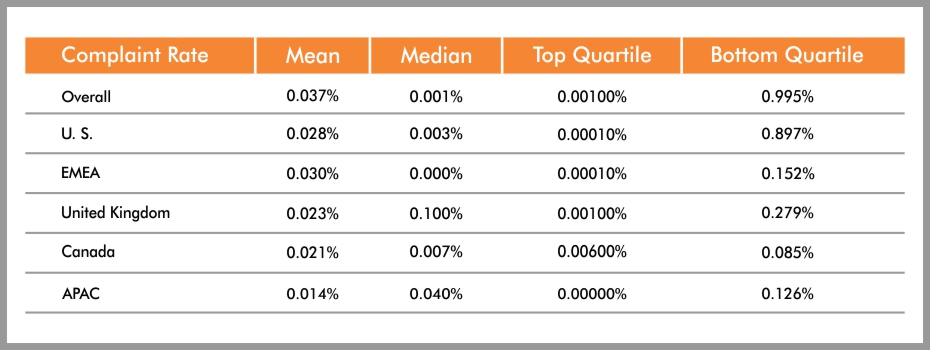
\includegraphics[width=\linewidth]{src/images/01-capitulo-1/representacion_tabla.jpg}
  \caption{Diagrama de representación en forma de tabla}
  \label{fig:representacion_tabla}
\end{figure}

\subsubsection*{Gráfico de barra}
Es una forma de representar gráficamente conjuntos de datos o valores, a través
del uso de barras rectangulares de longitudes proporcionales a los valores
representados. Son útiles para comparar elementos
(\autoref{fig:representacion_barras}).

\begin{figure}
  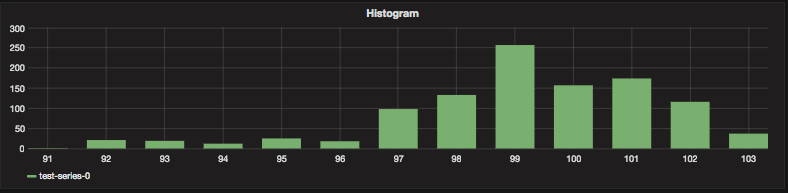
\includegraphics[width=\linewidth]{src/images/01-capitulo-1/representacion_barras.png}
  \caption{Diagrama de representación con barras}
  \label{fig:representacion_barras}
\end{figure}

\subsubsection*{Gráfico de línea}
Es una manera de visualizar información compuesta de una serie de datos
representados por puntos y unidos por segmentos lineales. Este tipo de gráficos
sirve para comprobar de forma sencilla la tendencia de los
datos.(\autoref{fig:representacion_lineas})

\begin{figure}
  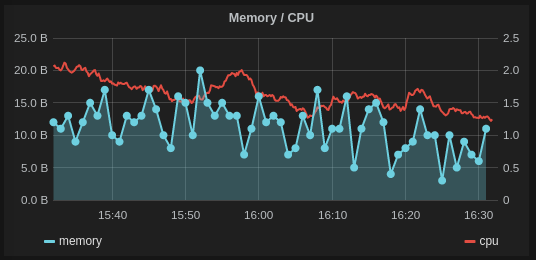
\includegraphics[width=\linewidth]{src/images/01-capitulo-1/representacion_lineas.png}
  \caption{Diagrama de representación con líneas}
  \label{fig:representacion_lineas}
\end{figure}

\subsubsection*{Gráfico circular}
También llamado gráfico de torta o \eng{pie chart}. Es un recurso estadístico
que se utiliza para representar porcentajes o proporciones. Consiste en dividir
a un círculo en secciones coloreadas, donde el tamaño de cada sección es
proporcional al valor que se intenta representar
(\autoref{fig:representacion_circular}).

\begin{figure}
  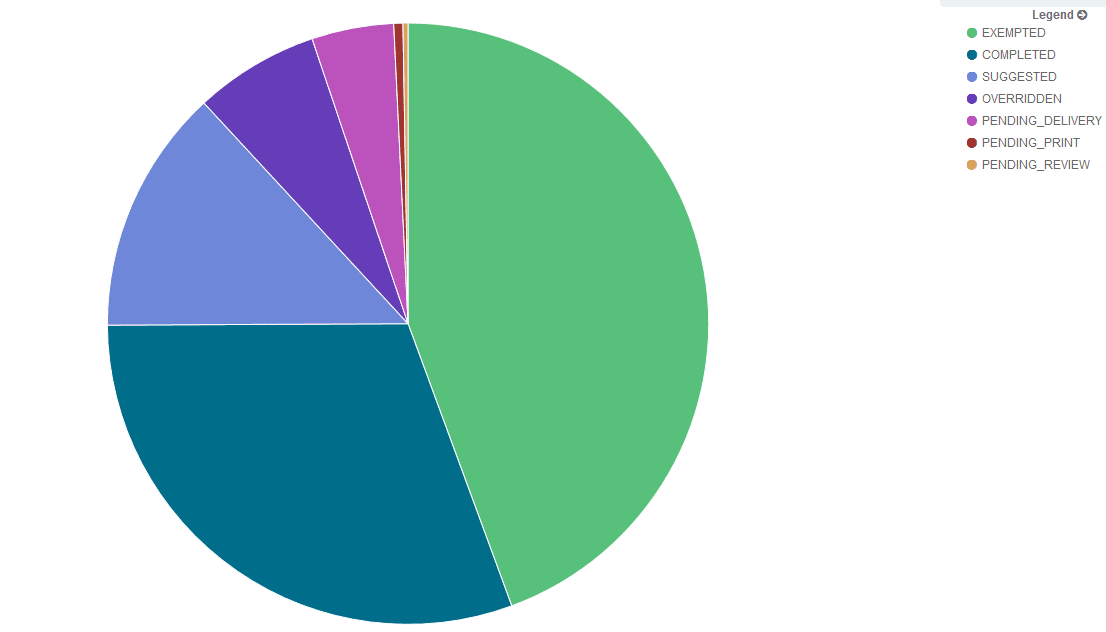
\includegraphics[width=\linewidth]{src/images/01-capitulo-1/representacion_circular.png}
  \caption{Diagrama de representación en forma circular}
  \label{fig:representacion_circular}
\end{figure}

\subsubsection*{Gráfico de dispersión}
También conocidos como \eng{Scatter Plot}, estos gráficos usan valores
numéricos para ambos ejes. Son útiles para mostrar la relación entre distintos
tipos de datos. Los gráficos de burbujas son una variación de este tipo de
gráficos, los puntos pueden ser de distintos tamaños, representando una
dimensión adicional a los datos (\autoref{fig:representacion_dispersion}).

\begin{figure}
  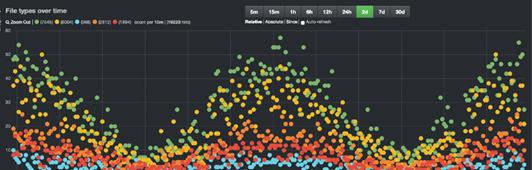
\includegraphics[width=\linewidth]{src/images/01-capitulo-1/representacion_dispersion.jpg}
  \caption{Diagrama de representación de dispersión}
  \label{fig:representacion_dispersion}
\end{figure}

A la hora de mostrar información es importante conocer las distintas maneras de
visualizar información, analizar qué es lo que se quiere transmitir y tener
criterio para decidir la forma en la que se mostrarán los datos.


\subsection{Alertas}
\label{alertas}

En las secciones anteriores hemos mencionado conceptos importantes en cuanto a
la obtención, manipulación, procesamiento, almacenamiento, resumen y
visualización de información de sistemas que proveen información valiosa.

En el libro Effective Monitoring and Alerting, el autor explica que con la
información generada a través de técnicas de monitorización es posible producir
un gran número de tableros a los cuales es importante prestarles atención.
Contratar personas para visualizar estos tableros no siempre es una tarea
rentable. Esta tarea no es muy gratificante, e incluso si lo fuera, es por lo
menos discutible que un operador humano sea mejor que una máquina o algoritmo
reconociendo patrones cuya atención pueda prevenir una situación no deseada
\cite[p. ~ 47]{monitoreo:efective_monitoring_and_alerting}.

Una alerta puede ser un mensaje enviado con el fin de notificar sobre un evento
importante a una persona. Este mensaje puede ser transmitido mediante correo
electrónico, servicio de mensajes simples, mensaje instantáneo, llamada
telefónica o a través de un servicio de notificaciones de alguna herramienta de
software.

Es deseable que un sistema de monitoreo tenga la capacidad de detectar aquellos
eventos significativos o que denoten un grave cambio de estado en el negocio,
aplicación o sistema, y puedo notificarlo a los interesados a través de un
sistema de alertas.

Los sistemas de alertas suelen ser configurados por los profecionales de
\gls{acro:it} para detectar y prevenir problemas. Las alertas pueden brindar
información sobre eventos no deseados, umbrales sobrepasados, caídas del
sistema o hitos alcanzados.

Las alertas deben ser transmitidas al destinatario adecuado, es decir, a una
persona que esté obligada a tratar con el evento.

Según Jason Dixon, autor de Monitoring with Graphite, para todos los propósitos
prácticos, alertar constituye el momento en que un sistema de monitoreo
identifica un fallo que requiere alguna acción adicional. En la mayoría de los
casos, el sistema está diseñado para enviar un correo electrónico a un miembro
del equipo de operaciones, pero conseguir que la alerta llegue a su destino no
suele ser tan simple como parece.

Por ejemplo, puede suceder que el destinatario esté fuera del rango de su
servicio celular, o que tenga la computadora apagada. Es por esto que la
programación de llamadas y el enrutamiento de notificaciones deben ser
incluidos en cualquier discusión de alertas.

A medida que una organización crece, es mayor el número de personas que pueden
resolver el problema notificado, pero, al mismo tiempo, la complejidad para
saber cómo planificar estas alertas aumenta.

En este punto entran en juego las herramientas de manejo de alertas. Las mismas
se encargan de administrar alertas y gestionar los avisos. Algunas incluso
permiten organizar un calendario de llamadas \cite[p. ~
17]{monitoreo:monitoring_with_grapfite}.

Las alertas son registradas a menudo en la forma de una petición o \eng{ticket}
en un sistema de \gls{term:its} (\eng{Issue Tracking System}).

Un \gls{term:its} es un paquete de software que administra y mantiene listas de
incidentes conforme son requeridos por una institución. Estos sistemas suelen
ser usados por personal de servicio al cliente para crear, actualizar y
resolver incidentes reportados por usuarios, empleados de la organización o
sistemas de alertas automatizados.

Stawek Ligus aconseja operar de acuerdo al principio de monitoreo extensivo y
de alerta selectiva. Esto significa identificar qué métricas son útiles para el
negocio y configurar alarmas para las series de tiempo a partir de indicadores
clave. El autor sugiere una lista de métricas a considerar como candidatas para
alertar:

\begin{itemize}
  \item Recursos:
    \subitem Retardo de red y pérdida de paquetes: para obtener la métrica de
    latencia se puede utilizar el comando \texttt{\gls{term:ping}} tanto a una
    dirección externa como a una dirección interna y registrar el tiempo de ida
    y vuelta de cada una. Además se puede utilizar la información de
    \texttt{\gls{term:ping}} para calcular la pérdida de paquetes.  Si el
    paquete llega con éxito se anota 0, y si no llega se anota 1. Calculando el
    promedio de estos valores se obtiene la pérdida de paquetes en términos
    porcentuales.
    \subitem Utilización de \gls{acro:cpu}: este valor sirve como indicador
    para el esfuerzo computacional de las operaciones. En un sistema
    \gls{term:linux} puede obtenerse analizando el directorio
    \texttt{/proc/stat}.
    \subitem Espacio disponible de disco y memoria: es importante evitar que el
    almacenamiento local se llene y que la cantidad de espacio libre en disco
    se aproxime a los límites. El uso excesivo del almacenamiento local puede
    inducir a un comportamiento impredecible para las aplicaciones.

  \item Plataforma:
    \subitem Tiempo de respuesta: puede ser útil extraer y registrar las
    estadísticas de tiempo de respuesta de los logs de las aplicaciones.
    Particularmente puede ser importante prestarle atención a los cambios en el
    promedio y a los \glspl{term:percentil}.
    \subitem Códigos de respuesta: registrar los códigos de errores
    \gls{acro:http} en aplicaciones \eng{web} es una buena idea si se
    quiere alertar sobre una proporción inusual de códigos \gls{acro:http}
    referidos a requerimientos erróneos o problemas del servidor.

  \item Aplicación:
    \subitem Disponibilidad: si se quiere lanzar una alerta cuando el
    porcentaje de solicitudes exitosas se encuentre debajo de un determinado
    umbral, es buena idea configurar controles de disponibilidad desde
    distintas ubicaciones, emitir solicitudes de prueba a cada minuto y
    registrar casos de éxito y de falla.
    \subitem Tasa de error: si se define de forma correcta aquello que
    constituye un error en las aplicaciones y se lo monitoriza muy de cerca, se
    puede decidir lanzar una alerta cuando estos errores suceden en una
    proporción relativamente alta.

\end{itemize}

\subsubsection*{Falsas alarmas}
\label{falsas_alarmas}

Un falso positivo es una alerta desencadenada por accidente o una mala
configuración. Estas alertas pueden ser molestas para los desarrolladores, y
además pueden conducirlos a desconfiar del sistema de monitoreo.

Si un programador tiene muchos falsos positivos, puede ocurrir que reste
importancia a las alertas y pierda información importante. Por ejemplo, un
sistema de alertas que envía gran cantidad de correos electrónicos con falsos
positivos puede hacer que el usuario desestime las alertas, deje de prestarles
atención y en consecuencia no actúe cuando ocurra un evento significativo que
necesite su atención inmediata.

Un falso negativo es una alerta que nuestro sistema de monitoreo no puede
detectar. Puede ser causada por el uso de umbrales inadecuados, por falta de
controles o por la utilización de intervalos de verificación de mucha o de muy
poca duración.

Los falsos negativos suelen ser identificados demasiado tarde, resultando por
ejemplo en la caída de un sistema o en la discontinuidad de la disponibilidad
de un servicio \cite[p.~16]{monitoreo:monitoring_with_grapfite}.

Es muy importante, a la hora de armar nuestra solución de alertas, tener muy
presenta estas situaciones y reducir al máximo el número tanto de falsos
positivos como negativos. Esto puede ser determinante para conseguir el éxito o
el fracaso de una solución propuesta.


  %   - Capítulo II
  \newpage
\section{Caso de estudio}
\label{cap2}

El equipo de trabajo de la oficina desarrolla, mantiene y da soporte a muchas
aplicaciones de diferentes dominios. La mayoría de estas aplicaciones son
implementadas usando los mismos lenguajes, librerías y tecnologías.

Algunas de las aplicaciones del \gls{acro:cespi} incluyen sistemas de manejo de
contenidos, sistemas administrativos de uso interno, un liquidador de sueldo y
otras aplicaciones al servicio de las necesidades de la \gls{acro:unlp}.

El \gls{acro:cespi} mantiene una gran cantidad de aplicaciones, algunas de las
cuales están escritas en el lenguaje de programación \gls{term:php} y otras en
el lenguaje \gls{term:ruby}. El gran número de aplicaciones en producción
complejizaba su mantenimiento, e hizo necesario comenzar a utilizar
herramientas que permitieran el manejo, instalación y aprovisionamiento de los
servidores de forma dinámica, escalable y consistente.

El incentivo del \gls{acro:cespi} por querer mejorar la infraestructura de
monitoreo en sus aplicaciones está estrechamente vinculado con su cultura de
trabajo. En la \autoref{cultura_de_trabajo} se explica en qué consiste esta
forma de trabajo, y de qué forma la aplicación de la cultura \gls{term:devops},
la estrategia \gls{term:lean} y la \gls{term:delivery_continuo} se vinculan con
la necesidad de mejorar su infraestructura de monitoreo de la oficina.

Con el objetivo de contextualizar el trabajo, en la
\autoref{tecnologias_utilizadas} se describe las herramientas y tecnologías
usadas en el \gls{acro:cespi}, se explicarán las características de la
infraestructura donde se despliegan las aplicaciones y los motivos de porqué
está implementada de esa manera. Además, se muestran algunas de las
particularidades que han sido tenidas en cuenta al diseñar nuestra solución de
monitoreo.

Finalmente en la \autoref{objetivos_de_nuestra_implementacion} se hace mención
las diferentes técnicas de monitoreo que se utilizan actualmente sobre las
aplicaciones explicando cuales son los objetivos buscados con la
implementación de la arquitectura de monitoreo propuesta.

\subsection{Cultura de trabajo}
\label{cultura_de_trabajo}

La forma de trabajo de la oficina está en constante evolución. Dedica tiempo y
esfuerzo en mejorar la calidad de las tareas que se realizan y la eficiencia en
la que se construyen los productos de \eng{software}. Hoy en día esta
metodología de trabajo se encuentra fuertemente inspirada en \gls{term:devops}.

\gls{term:devops} es una cultura de trabajo centrada en la comunicación,
colaboración e integración entre desarrolladores de \eng{software} y
profesionales de operaciones en tecnologías de información. Su objetivo es
ayudar a una organización a producir productos y servicios de \eng{software} de
forma rápida.

El \gls{acro:cespi} cuenta con un enfoque de trabajo de entregas continuas:
produce en cortos y frecuentes ciclos, asegurando que el \eng{software} pueda
ser desplegado de forma confiable en cualquier momento. Este enfoque ayuda a
reducir costos, tiempo y riesgos de cambios en las entregas al permitir más
actualizaciones incrementales en aplicaciones en producción.

El equipo de trabajo adquiere cada día más prácticas que tengan un enfoque
\gls{term:lean}. \gls{term:lean} es una manera de abordar el lanzamiento de
negocios y productos basada en el aprendizaje validado, experimentación e
iteración en los lanzamientos del producto para acortar los ciclos de
desarrollo, medir el progreso y ganar valiosa retroalimentación de parte de los
clientes.

Uno de los horizontes en cuanto a desarrollo a los que quiere llegar la oficina
es que las aplicaciones recorran el circuito \eng{lean startup} conocido como
“crear, medir y aprender”. Es un proceso iterativo que consiste en transformar
ideas en productos, medir el \eng{feedback} generado por los clientes a partir
del uso de la aplicación y aprender, a partir del análisis de la información
recolectada, para volver a repetir el ciclo.

Esta serie de ciclos comienza con la implementación de un producto mínimo
viable. Esto es, la versión de un nuevo producto que permite al equipo recoger
con el mínimo esfuerzo la máxima cantidad de conocimiento validado por los
consumidores de dicho producto.

La implementación de esta forma de trabajo permite al \gls{acro:cespi} comenzar un
proyecto con un gasto relativamente pequeño y ayudar a los programadores a
iniciar el proceso de aprendizaje sobre la aplicación de la forma más rápida
posible\cite[p~.2]{lean:the_lean_startup}.

Esta forma de trabajo permite que todos los involucrados en el desarrollo del
producto conozcan su ciclo de vida completo. Además incentiva la buena
documentación de la infraestructura y la disponibilidad de métricas para todos.

La filosofía de trabajo ha cumplido un papel fundamental en la promoción del
interés de los programadores y líderes de proyecto de la oficina en llevar a
cabo un monitoreo más adecuado de sus productos y servicios.

Esto es en parte así debido a que la medición constante de los datos de las
aplicaciones y los sistemas en general, demuestra ser invaluable a la hora de
tomar decisiones para contribuir a la mejora continua de dichas aplicaciones y
sistemas. La mejora contínua es uno de los pilares de la metodología de trabajo
de la oficina, y su relación con el monitoreo es una de las razones principales
por las que decidimos comenzar este trabajo.

\subsection{Tecnologías utilizadas en la oficina}
\label{tecnologias_utilizadas}

La oficina del \gls{acro:cespi} utiliza el \eng{framework} \eng{web}
\gls{term:ror}\footnote{Cf.  \url{http://rubyonrails.org/}} como principal
herramienta de desarrollo. Este framework fue elegido por su excelente
documentación, activa comunidad, facilidad para desarrollar e implementado en
el lenguaje Ruby.

Ruby, como se menciona en su sitio oficial, es un lenguaje creado con el
objetivo de ser “el mejor amigo del desarrollador”. Es orientado a objetos y su
sintaxis es muy amigable en comparación a otros lenguajes de programación. La
expresividad del lenguaje permite escribir código conciso, expresivo y fácil de
mantener.

\gls{term:ror} cuenta con soporte para las distintas bases de datos que se
utilizan en la oficina. Entre ellas se encuentran \gls{term:mysql},
\gls{term:mongo}, \gls{term:elasticsearch} y \gls{term:redis}.

La oficina se encuentra en transición a una arquitectura basada en contenedores
de \gls{term:docker}.

Docker es un proyecto de código abierto para la automatización del despliegue
de aplicaciones dentro de \glspl{term:contenedor} de \eng{software} en Linux.
Los contenedores proporcionan una capa adicional de abstracción y
automatización de virtualización a nivel de sistema operativo.

En el marco de la cultura de trabajo \gls{term:devops} del \gls{acro:cespi} se
decidió utilizar Docker para facilitar la construcción de una infraestructura
dinámica, escalable y tolerante a fallos que permitiera el despliegue seguro y
automático de aplicaciones, al mismo tiempo que redujera la brecha entre
desarrolladores de \eng{software} y profesionales de operaciones en tecnologías
de información.

El manejo de múltiples \glspl{term:contenedor} de \gls{term:docker} en
producción se convirtió en una tarea compleja para la oficina, por lo que se
decidió utilizar \gls{term:rancher}. \gls{term:rancher} es una plataforma de.
código abierto que facilita la orquestación, disponibilidad, configuración y
enlace de \glspl{term:contenedor} de \gls{term:docker}. Esta herramienta
permite resolver gran parte de los desafíos críticos presentes al ejecutar
aplicaciones en \glspl{term:contenedor} de \gls{term:docker}.

Rancher provee un conjunto completo de servicios de infraestructura para
contenedores, incluyendo herramientas de red, servicios de almacenamiento de
imágenes de \glspl{term:contenedor} privadas, administración de los hosts que forman parte
de la infraestructura, facilidades para el despliegue, balanceo de carga y
sencillas herramientas de monitoreo.

\subsection{Objetivo de nuestra implementación}
\label{objetivos_de_nuestra_implementacion}

Creemos importante construir una infraestructura de monitoreo que nos permita
obtener valiosa información sobre las reglas de negocio de las aplicaciones que
se desarrollan en la oficina, de forma que permita al equipo de trabajo contar
con datos duros para tomar decisiones de negocio más confiables.

Además, los desarrolladores del \gls{acro:cespi} creen que sería útil contar con
una herramienta de recolección y análisis de información sobre el rendimiento de
las aplicaciones. Esta herramienta podría ayudar a encontrar puntos débiles y
cuellos de botella en las aplicaciones.

A las personas encargadas de mantener la infraestructura de la oficina les
interesa tener un seguimiento de datos de uso del sistema operativo y las
computadoras, como el uso de \gls{acro:cpu}, la cantidad de memoria utilizada y
disponible, número de tareas en espera, uso de la memoria \gls{term:swap},
cantidad de procesos, espacio utilizado en disco.

Anteriormente los desarrolladores no contaban con una implementación formal de
monitoreo, sino que recurrían a diversas técnicas para llevar a cabo el
seguimiento de las aplicaciones, detectar errores y prevenir su aparición.

Una de las técnicas utilizadas por el grupo de desarrollo era la búsqueda y
lectura de registros de logs de forma manual. El programador se conectaba a
través de \gls{term:ssh} al servidor de la aplicación y visualizaba los logs
directamente mediante la consola.

Si el desarrollador requería conocer información en tiempo real de los recursos
del servidor donde estaban corriendo las aplicaciones, éste debía conectarse al
servidor y ver la información utilizando el comando \gls{term:htop}.

Para obtener una devolución del funcionamiento de las consultas a bases de
datos se utilizaba una herramienta que permitía configurar el envío de reportes
a través de correo electrónico usando la funcionalidad
\texttt{slow\_query\_log} provista por \gls{term:mysql}. Esta funcionalidad
guarda información de consultas que toman mucho tiempo en llevarse a cabo. Este
tiempo es por defecto de 10 segundos, pero puede ser definido por un usuario.

Para ser notificados de errores en producción de las aplicaciones
\gls{term:ror}, los programadores hacían uso de la \gls{term:gema} Exception
Notifier\footnote{Cf.
\url{https://github.com/smartinez87/exception_notification}}. Esta librería
permite configurar en el código de la aplicación, una dirección de correo para
recibir las notificaciones de errores en la aplicación, y se acciona cuando la
aplicación devuelve a un usuario un código \gls{acro:http} de error.

La notificación cuenta con valiosa información del contexto de la aplicación.
Algunos ejemplos son el tipo de solicitud, los datos de la sesión del usuario,
los parámetros de la petición y también el \gls{term:stack_trace}, que contiene
información de las llamadas a los métodos que dieron origen al error.

Para realizar recolección, análisis de datos y generación de alertas, en la
oficina se utiliza las herramientas de monitoreo \gls{term:graphite} y Nagios.

Graphite es una herramienta libre y de código abierto que sirve para monitorear
y graficar la performance de sistemas de computadoras. \gls{term:graphite} recolecta,
almacena y muestra datos de tipo time-series en tiempo real.

Nagios es una aplicación libre y de código abierto que monitoreo sistemas,
redes e infraestructura. Nagios ofrece monitoreo y servicios de alertas para
servidores, \eng{switches}, aplicaciones y servicios.

Uno de los problemas que identificamos como consecuencia del uso de estas
técnicas es que estos mecanismos generan una notificación cada vez que ocurría
un error. Por lo que si un error ocurría cientos de veces en un día, el usuario
recibiría cientos de mensajes idénticos.

Partiendo del conocimiento que obtuvimos con nuestra primera investigación,
creímos importante ayudar a mejorar la forma en que se implementaba el
monitoreo en el \gls{acro:cespi}.

La oficina podría beneficiarse con una infraestructura de monitoreo que brinde
información útil a los usuarios, sea fácil de utilizar, pueda adaptarse a una
arquitectura de \glspl{term:contenedor} y sea dinámica y escalable.

Nuestro primer paso para implementar la nueva infraestructura de monitoreo será
recolectar métricas en tiempo real que provengan del uso de las aplicaciones y
los \glspl{term:contenedor}, y obtener de ellos valiosa información que nos
permita prevenir errores y tomar mejores decisiones de diseño.

Luego buscaremos utilizar la información que brindan los logs de forma más
intensiva. Unificar el formato de los logs y centralizar los logs que provengan
de diversas fuentes en un único lugar.

La infraestructura de aplicaciones y servicios que queremos monitorear es
dinámica, escalable, construida de forma automatizada y creada a partir de
código reutilizable. Intentaremos lograr una forma de monitoreo que pueda
adaptarse a las características de esta infraestructura, por lo que
investigaremos cómo utilizar \glspl{term:contenedor} de \gls{term:docker} para
implementar algunos componentes del sistema de monitoreo.

Con el objetivo de impulsar un sistema que brinde información útil a los
usuarios, trataremos de aplicar algunas de las técnicas de visualización
efectiva mencionadas en el capítulo anterior
(\autoref{visualizacion-efectiva}) durante la creación de tableros con
gráficos.

Finalmente, nos ocuparemos de implementar una solución de alertas de mayor
utilidad que evite, en la medida de lo posible, falsos positivos y negativos y
brinde notificaciones útiles a los usuarios indicando concretamente el problema
y/o ayudándolos a prevenirlos.

En los próximos capítulos explicaremos la forma en que desarrollamos una
infraestructura de monitoreo que intente cumplir con las características
mencionadas.



  %   - Capítulo III
  \newpage
\section{Almacenamiento de series de tiempo}
\label{cap3}

En este capítulo explicaremos cómo hemos logrado recolectar, almacenar y
consultar información generada en tiempo real de varias fuentes. Ejemplos de
esta información son el uso del disco rígido, los procesadores y la memoria.

En la sección 3.1 repasaremos las características que tienen los datos generados
en tiempo real, y describiremos brevemente algunas herramientas que permiten el
almacenamiento y consulta de estos datos de forma eficiente. En particular
explicaremos qué es InfluxDB y cómo configurarlo.

En la sección 3.2 demostraremos cómo obtener información valiosa de las
aplicaciones \gls{term:ror} a partir de la instrumentación y daremos una
introducción a la librería influxdb-rails, que nos permitirá enviar datos
tomados de las aplicaciones a nuestra instancia de InfluxDB.

En la sección 3.3 mostraremos herramientas que nos permitan obtener información
del funcionamiento en tiempo real de contenedores de \gls{term:docker}. En
particular desarrollaremos cómo configurar la herramienta cAdvisor para enviar
información de los contenedores a InfluxDB.

En la sección 3.4 mostraremos cómo se pueden utilizar las herramientas que hemos
configurado a lo largo del capítulo para almacenar y consultar datos a InfluxDB
a través de su cliente web.

\subsection{Almacenamiento}
\label{almacenamiento}

En la sección 1.2 hemos descrito las particularidades que tienen los datos de series de tiempo. Una de estas particularidades es que todas las series de tiempo comparten entre sí una dimensión: la dimensión de tiempo, y por eso son útiles para correlacionar datos de varias fuentes.

Las bases de datos relacionales tradicionales pueden no ser prácticas para manejar almacenar estos tipos de datos. Una base de datos de series de tiempo es un sistema de software que está optimizado para manejarlos de forma correcta, confiable y eficiente.

@book{book:1567575,
   title =     {Time Series Databases  New Ways to Store and Access Data},
   author =    {Ted Dunning, Ellen Friedman},
   publisher = {O'Reilly Media},
   isbn =      {},
   year =      {2014},
   series =    {},
   edition =   {},
   volume =    {},
   url =       {http://gen.lib.rus.ec/book/index.php?md5=5BCDBD7931F770AA509E5D9D27C7A978}}


Hemos analizado las herramientas InfluxDB y Graphite para almacenar datos de este tipo. 

InfluxDB es una base de datos de código abierto implementada en el lenguaje Go con el propósito de manejar datos de series de tiempo con requerimientos de gran disponibilidad y alto rendimiento. InfluxDB no tiene dependencias externas.

InfluxDB viene con una API HTTP integrada, lo que permite que no sea necesario escribir ningún código del lado de servidor para comenzar a trabajar.
https://github.com/influxdata/influxdb

Es posible etiquetar los datos, lo que permite una consulta muy flexible. Esta consulta se escribe en un lenguaje similar a SQL, llamado InfluxQL.  https://docs.influxdata.com/influxdb/v0.9/query_language/query_syntax/

InfluxDB permite contestar consultas en tiempo real, lo que significa que cada valor se indexa a medida que llega y está disponible casi inmediatamente para su uso.

Graphite es una herramienta de monitoreo capaz de ser ejecutada en una amplia gama de computadoras, y también en la nube. Graphite es usado para tener un seguimiento del rendimiento de sitios web, aplicaciones, servicios de negocio y servidores en una red.

Con Graphite es relativamente sencillo almacenar, recuperar, compartir y visualizar datos de tipo series de tiempo.

Graphite consiste en tres componentes de software:
carbon: Un servicio de alto rendimiento que recepta datos de tipo series de tiempo
whisper: Una base de datos sencilla para almacenar datos de tipo series de tiempo
graphite-web: Una interfaz de usuario y API para visualizar gráficos y tableros.

Las métricas son alimentadas a través del servicio Carbon, que envía datos a las bases de datos Whisper para su almacenamiento a largo plazo. Los usuarios interactúan con la interfaz de graphite-web o con su API, que a su vez consulta a Carbon y Whisper por los datos necesarios para construir los gráficos requeridos.

La plataforma web de Graphite ofrece una variedad de estilos y formatos de salidas, incluyendo imágenes, archivos separados por comas, XML y JSON. 

http://graphite.readthedocs.io/en/latest/overview.html

OpenTSDB es una base de datos de series de tiempos distribuida y escalable, escrita sobre HBase. OpenTSDB almacena, indexa y sirve métricas recolectadas de sistemas de computadoras, como por ejemplo redes, sistemas operativos y aplicaciones, a gran escala, y hace que estos datos sean accesibles y graficables de forma fácil.

OpenTSDB permite recolectar métricas de hosts y aplicaciones a una taza de tiempo alta y es capaz de recolectar miles de métricas de decenas de miles de hosts y aplicaciones, y almacenar miles de millones de valores estadísticos.

OpenTSDB es software libre y está disponible en ambas licencias LGPLv2.1 + GPLv3
Find more about OpenTSDB at http://opentsdb.net

Finalmente hemos elegido InfluxDB para nuestra implementación por sobre las demás herramientas. La decisión no fue fácil, ya que todas las herramientas nos parecieron muy prometedoras. La razón por la que elegimos InfluxDB es que nos pareció que esta herramienta tenía mejor soporte para el lenguaje Ruby que las alternativas. Además, creímos que el hecho de que InfluxDB tenga un lenguaje de consulta similar a SQL facilitaría el desarrollo de consultas al personal de la oficina.

InfluxDB es fácil de instalar y administrar.

Puede ser instalado usando uno de sus paquetes pre armados para diferentes sistemas operativos. https://portal.influxdata.com/downloads. Para instalar InfluxDB versión 1.2 en una distribución Linux basada en Debian, basta con correr los siguientes comandos en una terminal:


wget https://dl.influxdata.com/influxdb/releases/influxdb_1.2.0_amd64.deb
sudo dpkg -i influxdb_1.2.0_amd64.deb

Luego, para ejecutar el programa basta con correr el comando service influxdb start.

Una vez que InfluxDB está instalado, es posible crear una base de datos, insertar datos y realizar consultas usando la API de InfluxDB. Incluso se puede hacer todo esto desde la consola usando el comando curl:

1- Crear una base de datos de nombre monitoreo:

curl -XPOST 'http://localhost:8086/query' --data-urlencode "q=CREATE DATABASE monitoreo"

2- Insertar algunos datos:

curl -XPOST 'http://localhost:8086/write?db=monitoreo \
-d 'cpu,host=server01,region=uswest load=42 1434055562000000000'

curl -XPOST 'http://localhost:8086/write?db=monitoreo \
-d 'cpu,host=server02,region=uswest load=78 1434055562000000000'

curl -XPOST 'http://localhost:8086/write?db=monitoreo \
-d 'cpu,host=server03,region=useast load=15.4 1434055562000000000'


3- Consultar los datos:

curl -G http://localhost:8086/query?pretty=true --data-urlencode "db=monitoreo" \
--data-urlencode "q=SELECT * FROM cpu WHERE host='server01' AND time < now() - 1d"

curl -G http://localhost:8086/query?pretty=true --data-urlencode "db=monitoreo" \
--data-urlencode "q=SELECT mean(load) FROM cpu WHERE region='uswest'"

InfluxDB utiliza varios puertos de red para funcionar. Todos los mapeos de puertos pueden ser modificados en el archivo de configuración que suele estar localizado en /etc/influxdb/influxdb.conf.

Por defecto, InfluxDB usa los siguientes puertos de red:
El puerto TCP 8086 es usado para la comunicación entre cliente y servidor sobre la API HTTP de InfluxDB
El puerto TCP 8088 es usado para el servicio RPC de backup y restauración.

Además de estos puertos, InfluxDB ofrece múltiples plugins que pueden requerir puertos personalizados. 


  %   - Capítulo IV
  \newpage
\section{Almacenamiento de logs}
\label{cap4}

Para implementar la nueva infraestructura de monitoreo, y con el objetivo de
darles uso real a los registros de las aplicaciones, nuestro primer paso será
intentar utilizar la información que brindan los logs de forma más intensiva.

En \gls{term:ror}, los logs son complejos. Cada registro puede ocupar varias
líneas, y cada tipo de log tiene su propio formato. En la sección 4.1
explicaremos cómo extraer valiosa información de los logs de las aplicaciones
del laboratorio.

Utilizaremos los logs de \gls{term:nginx} para recolectar datos precisos sobre
la velocidad de respuesta de las aplicaciones ante solicitudes \eng{web}.
En la sección 4.2 explicaremos cómo configurar la herramienta para que la
información recolectada sea útil en un ambiente de trabajo con contenedores de
\gls{term:docker}.

Para poder hacer uso de la información de los registros de ambas fuentes,
necesitaremos algún tipo de herramienta de almacenamiento y búsqueda. En el
capítulo 4.3 describiremos cómo configurar \gls{term:elasticsearch} como motor
de búsqueda y análisis de logs.

En la sección 4.4 explicaremos cómo unificar los logs de diversas fuentes y
cómo centralizarlos en un la base de datos descripta en el capítulo anterior.
Utilizaremos \gls{term:fluentd} para lograr que las aplicaciones y las
instancias de \gls{term:nginx} se comuniquen correctamente con
\gls{term:elasticsearch}, y mostraremos cómo configurarlo.

Una vez que tengamos todo el sistema de recolección, unificación,
centralización y almacenamiento de logs configurado, demostraremos cómo obtener
información útil a través de una \gls{term:api} y utilizando un lenguaje de
consultas. En la sección 4.5 daremos algunos ejemplos de uso del sistema
construido en funcionamiento.

\subsection{Configuración de las aplicaciones}
\label{configuracion_de_las_aplicaciones}

Para poder hacer uso de los logs de nuestras aplicaciones, debimos tener en
cuenta que la oficina se encuentra en un proceso de migración de
infraestructura a contenedores de \gls{term:docker}.

La manera recomendada en la documentación de \gls{term:docker} para realizar
logging, es imprimiendo los logs de nuestras aplicaciones en el
\gls{acro:stdout} \footnote{Cf.
\url{https://docs.docker.com/engine/admin/logging/view_container_logs/}}.  Es
por ello que debimos configurar los logs de nuestras aplicaciones para que sean
escritos en la salida estándar. Utilizar esta estrategia nos permite contar
con información del contenedor en ejecución, como lo son su identificador y su
nombre.

\gls{term:docker} tiene soporte para múltiples mecanismos de logging. Al
iniciar el daemon de \gls{term:docker} se puede usar la bandera
\texttt{--log-opt NAME=VALUE} para especificar el driver para realizar logging
que usará por defecto el contenedor.

Para este trabajo utilizaremos otra forma de configurar el driver, que es a
través de la opción \texttt{log-driver=VALUE} durante el comando
\gls{term:docker}
run\footnote{\url{https://docs.docker.com/engine/admin/logging/overview/}}.

Una vez hecho esto, el siguiente paso es configurar nuestras aplicaciones para
que envíen sus logs a la salida estándar.

Por defecto \gls{term:ror} mantiene un archivo separado para los logs por cada
ambiente de ejecución, y para hacer uso de la información de los logs utiliza
la clase \texttt{ActiveSupport::Logger}. Aunque \gls{term:ror} viene con una
configuración para el manejo de log predeterminada, puede puede cambiarse la
misma especificando un logger alternativo en un archivo de configuración de la
siguiente forma:

\begin{lstlisting}

config.logger = SomeLogger

\end{lstlisting}

Podemos lograr que \gls{term:docker} capture correctamente los logs de
\gls{term:ror} agregando la siguiente especificación al archivo
config/application.rb de la aplicación:

\begin{lstlisting}

config.logger = ActiveSupport::Logger.new(STDOUT)

\end{lstlisting}

Los logs de \gls{term:ror} tienen algunas características que hacen que sea
difícil trabajar con ellos. En primer lugar, no siguen un formato estándar.
Esto hace que para distintos tipos de logs sea necesario usar diferentes
estrategias para recuperar la información valiosa. En segundo lugar, un solo
log puede ocupar varias líneas, lo que hace complejo identificar dónde termina
un log y dónde empieza el siguiente.

Para resolver estos problemas utilizamos una gema llamada lograge\footnote{Cf.
\url{https://github.com/roidrage/lograge}}. Esta gema se encarga de transformar
complejos logs multilínea de \gls{term:ror} en simples logs con datos
importantes bien identificados de una sola línea.

Por ejemplo, un log de \gls{term:ror} se ve de la siguiente manera:

\begin{lstlisting}

Started GET "/" for 126.0.0.1 at 2012-03-10 14:28:14 +0100
Processing by HomeController#index as HTML
  Rendered text template within layouts/application (0.0ms)
  Rendered layouts/_assets.html.erb (2.0ms)
  Rendered layouts/_top.html.erb (2.6ms)
  Rendered layouts/_about.html.erb (0.3ms)
  Rendered layouts/_google_analytics.html.erb (0.4ms)
Completed 200 OK in 79ms (Views: 78.8ms | ActiveRecord: 0.0ms)

\end{lstlisting}

Usando lograge, el mismo log se transforma en:

\begin{lstlisting}

method=GET path=/jobs/833552.json format=json controller=JobsController  action=show status=200 duration=58.33 view=40.43 db=15.26

\end{lstlisting}

Para configurar lograge en la aplicación \gls{term:ror}, debe incluirse la gema
con el mismo nombre a la lista de dependencias de la aplicación. Para hacerlo
basta con agregar la siguiente línea de código al archivo \texttt{Gemfile}:

\begin{lstlisting}

gem 'lograge'

\end{lstlisting}

Luego debe agregarse en el archivo \texttt{config/application.rb} la siguiente
especificación:

\begin{lstlisting}

class Application < Rails::Application
  config.logger = ActiveSupport::Logger.new(STDOUT)
  config.log_formatter = nil
  config.log_level = :info

  config.lograge.enabled = true
  config.lograge.formatter = Lograge::Formatters::Json.new
  config.lograge.custom_options = lambda do |event|
    {
      app_timestamp: event.time
    }
  end
end

\end{lstlisting}

Con estas configuraciones ya contamos con una aplicación \gls{term:ror} que
envía la información de sus logs a la salida estándar en un formato más fácil
de procesar posteriormente.



  %   - Capítulo V
  \newpage
\section{Visualización}
\label{cap5}

La visualización de datos es el proceso de interpretación, contratación y comparación de datos que permite un conocimiento en profundidad y detalle de los mismos de tal forma que se transformen en información comprensible para las personas.

En la sección 5.1 explicaremos qué son las herramientas de visualización de datos y describiremos las herramientas Kibana y Grafana.

En la sección 5.2 explicaremos como configurar Kibana para realizar consultas en nuestra instancia de Elasticsearch. Además mostraremos cómo crear gráficos a partir de estos datos y de qué forma explorar los logs desde el cliente web de Kibana.

En la sección 5.3 mostraremos cómo instalar y configurar Grafana para que trabaje de forma correcta con InfluxDB. Configuraremos un datastore vinculado con nuestra instancia de InfluxDB y crearemos tableros con gráficos que hagan uso de esta información.

\subsection{Herramientas}
\label{herramientas-de-visualizacion}

Las herramientas de software de visualización de datos son aquellas que ocupan
de mostrar datos de distintas fuentes en forma de gráficos, de forma que los
usuarios puedan descubrir patrones y entender la información de forma sencilla.

Existen varias herramientas informáticas para visualizar datos. En esta sección
describiremos brevemente a las herramientas \gls{term:kibana} y
\gls{term:grafana}.

\gls{term:kibana} es una plataforma de análisis y visualización de código
abierto diseñada para trabajar con \gls{term:elasticsearch}. Se lo puede usar
para buscar, observar e interactuar con datos almacenados en índices de
\gls{term:elasticsearch}.

Con \gls{term:kibana} es posible realizar análisis de datos complejos y
visualizar datos en una variedad de gráficos, tablas y mapas.
\autoref{fig:kibana}


\begin{figure}
  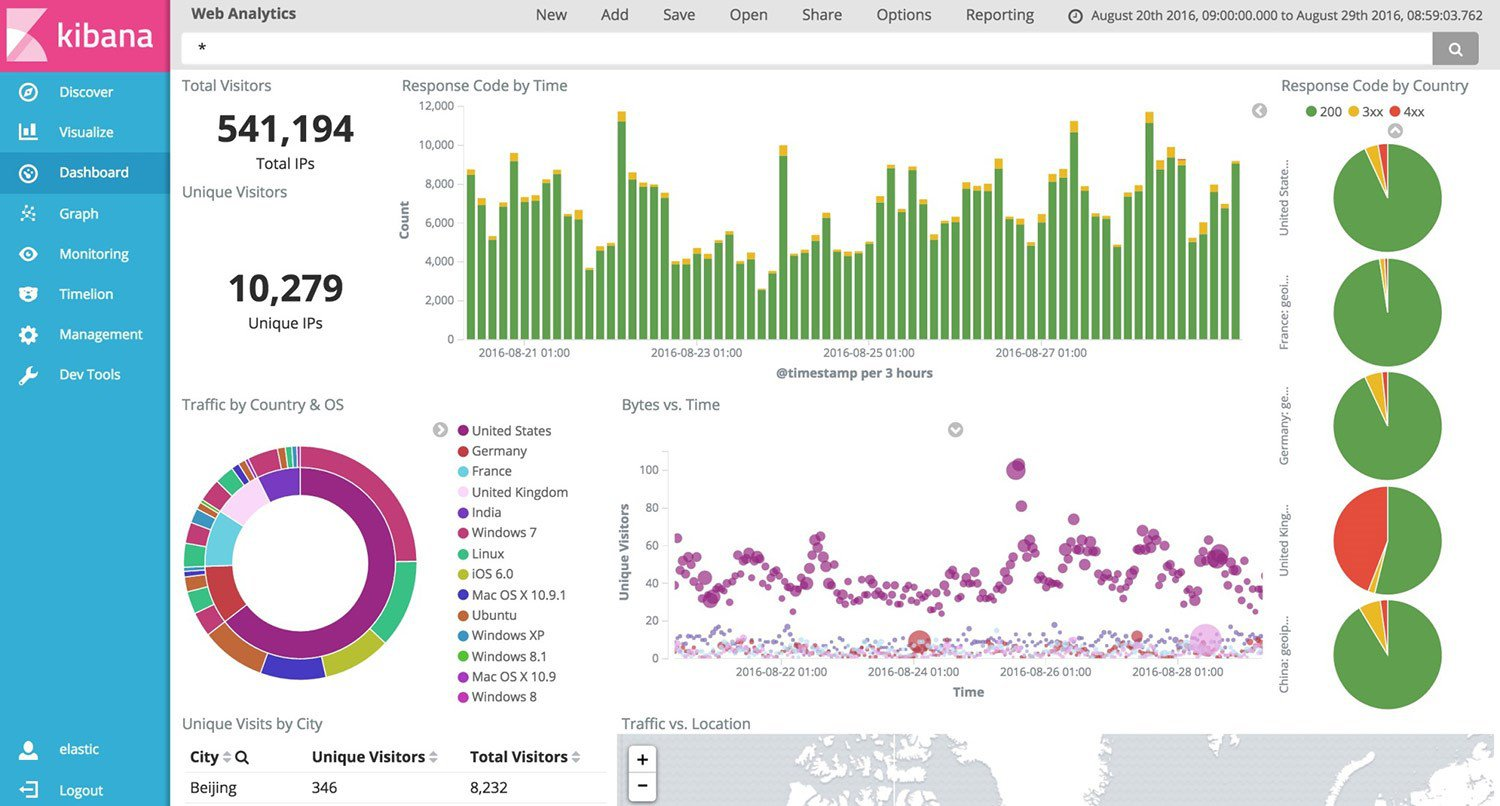
\includegraphics[width=\linewidth]{src/images/05-capitulo-5/kibana.jpg}
  \caption{Tablero de \gls{term:kibana}}
  \label{fig:kibana}
\end{figure}

\gls{term:kibana} cuenta con una interfaz basada en el navegador, que permite
crear y compartir tableros de control dinámicos que muestran los cambios a
consultas de \gls{term:elasticsearch} en tiempo real.

Como hemos mencionado en la teoría, el contar con formas visuales de
representar información permite a las personas entender grandes volúmenes de
datos de forma más sencilla.

\gls{term:grafana} es un tablero y componedor de gráficos de propósito general
y de código abierto que corre como una aplicación \eng{web}. Es comúnmente
usado para visualizar datos de series de tiempo para infraestructuras en la
\eng{web} y analíticas de aplicación, pero también es usado en sensores
industriales, automatización de viviendas, medición del clima y control de
procesos.\autoref{fig:grafana}

\begin{figure}
  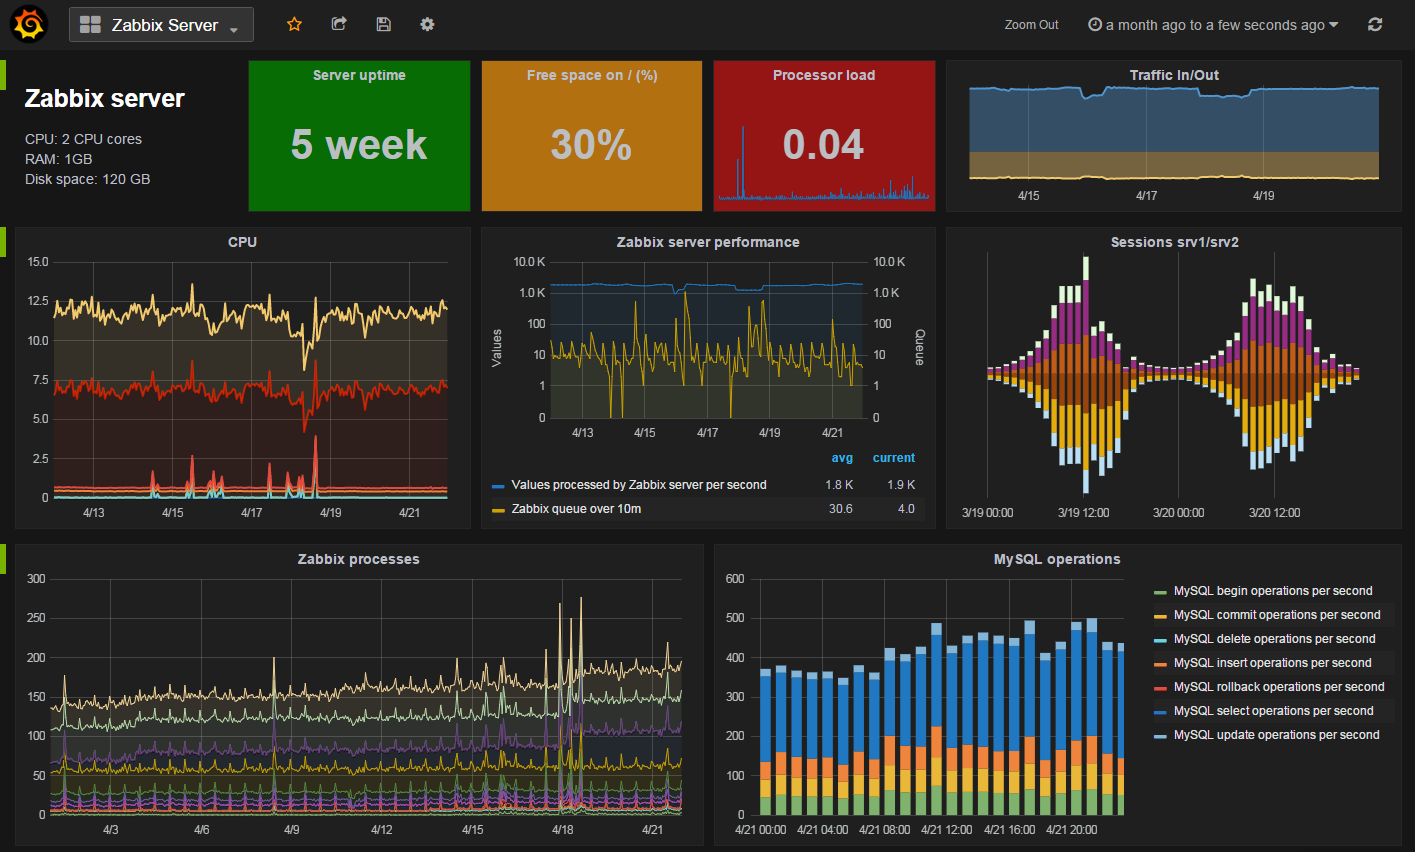
\includegraphics[width=\linewidth]{src/images/05-capitulo-5/grafana.png}
  \caption{Tablero de \gls{term:grafana}}
  \label{fig:grafana}
\end{figure}

\gls{term:grafana} permite una sencilla extensibilidad y variedad de paneles,
con ricas opciones de visualización, y tiene soporte para las fuentes de datos
de series de tiempo más populares, incluyendo \gls{term:influx} y
\gls{term:elasticsearch}.

Luego de analizar estas opciones, nos pareció que la herramienta de
visualización más completa entre ambas era \gls{term:grafana}.

Pero \gls{term:kibana} es un front-end de elasticsearch y está preparado
especialmente para realizar consultas sobre esta base de datos de forma simple.
Con \gls{term:kibana} es posible hacer consultas directas sobre los registros
de logs tal cual fueron recuperados e indexados.

Es por esto que decidimos usar ambas herramientas: \gls{term:kibana} para
consultar las base de datos de \gls{term:elasticsearch}, y hacer consultas
acerca de los logs, y \gls{term:grafana} para comunicarse con nuestra instancia
de \gls{term:influx} y visualizar datos generados en tiempo real.

Creemos importante destacar que estas herramientas están en constante
crecimiento, por lo que no descartamos que en un futuro \gls{term:grafana}
incorpore funcionalidades que se encuentren presentes en \gls{term:kibana}, y
viceversa.


  %   - Capítulo VI
  \newpage
\section{Alertas}
\label{cap6}

Cómo mencionamos en la \autoref{alertas}, las alertas nos brindan la
posibilidad de ser notificados de forma automática sobre eventos que nos
parecen importantes.  Si no se cuenta con un sistema de alertas, la mejor forma
de identificar un problema es visualizar el funcionamiento de las aplicaciones,
de forma constante y manual.

Esto puede ser muy costoso, y es uno de los motivos por los que la elección de
una herramienta de generación de alertas que nos permita describir las
condiciones que deben complirse para ser notificados de situaciones importantes
se torna fundamental.

En este capítulo describiremos las herramientas que nos han parecido más
adecuadas para resolver la importante tarea de las alertas, al mismo tiempo que
daremos las razones de estas elecciones. Además mostraremos cómo configurar
estas herramientas para ser notificados de eventos importantes que ocurran en
la infraestructura.

En la \autoref{eleccion-herramienta} describiremos la herramienta
\gls{term:kapacitor}, que permite la definición de alertas y el envío de las
mismas a distintas fuentes, y explicaremos cómo instalarla y configurarla para
generar importantes alertas.

En la \autoref{definir-alerta} demostraremos cómo utilizar el lenguaje
\gls{term:tick_script} para definir alertas. Primero con un ejemplo sencillo, y luego con
un ejemplo más complejo.

En la \autoref{manejador-alertas} explicaremos los problemas encontrados en la
generación de múltiples alertas y cómo lo hemos solucionado utilizando la
herramienta de nombre \gls{term:alerta}.


\subsection{Elección de la herramienta y funcionamiento}
\label{eleccion-herramienta}

Hemos elegido la herramienta \gls{term:kapacitor} para implementar las alertas
en nuestra solución. Las razón detrás de nuestra decisión es que
\gls{term:kapacitor} cuenta con una \gls{acro:dsl} realmente simple, la cual
nos ha permitido implementar algunas alertas complejas de forma verdaderamente
rápida. Además, el hecho de que haya sido desarrollado por la misma empresa
que creó \gls{term:influx} le ha otorgado una integración excelente con el
mismo.

\gls{term:kapacitor} es un framework de procesamiento de datos de código
abierto, que permite crear alertas, correr procesos ETL (de extracción,
transformación y carga) y detectar anomalías. \gls{term:kapacitor} es parte del
\eng{stack} TICK, junto con Telegraf, \gls{term:influx} y Chronograf.

\gls{term:kapacitor} permite procesar datos por streaming y por lotes. También
consultar los datos de \gls{term:influx} en un programa y recibir datos a
través del protocolo de línea y cualquier otro método que \gls{term:influx}
admita.

Adicionalmente, admite realizar cualquier transformación actualmente posible en
el lenguaje de consulta InfluxQL y almacenar los datos transformados en
\gls{term:influx}. Además permite añadir funciones personalizadas definidas por
el usuario para detectar anomalías.

\gls{term:kapacitor} puede ser configurado para notificar alertas a distintos
destinos.  Por ejemplo se pueden enviar a un archivo de logs, una URL con
método \gls{acro:http} POST, a través de correo electrónico y servicios como
HipChat, \gls{term:alerta}, Sensu, Slack y PagerDuty, entre otros. Incluso es
posible ejecutar un comando dirigiendo los datos de la alerta por
\gls{acro:stdin}\footnote{\url{https://docs.influxdata.com/kapacitor/v1.2/}}.

\gls{term:kapacitor} cuenta con una \gls{acro:dsl} llamada TICKscript para
generar alertas. Esta \gls{acro:dsl} es usada para definir canales de
procesamiento de datos en \gls{term:kapacitor}.

\gls{term:kapacitor} usa este lenguaje para definir canales de procesamiento de
datos, o pipelines. Un pipeline es un conjunto de nodos que procesa datos y
aristas que conectan nodos. Los pipelines en \gls{term:kapacitor} son grafos
acíclicos dirigidos, lo que significa que cada arista tiene una dirección en la
que fluyen los datos y no puede haber ningún ciclo en el pipeline.

\gls{term:kapacitor} puede ser descargado e instalado en Debian o Ubuntu con
los siguientes comandos:

\begin{lstlisting}

wget https://dl.influxdata.com/kapacitor/releases/kapacitor_1.2.0_amd64.deb
sudo dpkg -i kapacitor_1.2.0_amd64.deb

\end{lstlisting}

Para correr el servicio de \gls{term:kapacitor} simplemente es necesario
ejecutar el siguiente comando en la terminar:

\begin{lstlisting}

sudo service kapacitor start

\end{lstlisting}

Además, es posible usarlo como \gls{term:contenedor} de \gls{term:docker}, a través de la
imágen oficial de \gls{term:kapacitor}
\footnote{\url{https://hub.docker.com/_/kapacitor/}}, con el comando:

\begin{lstlisting}

docker pull kapacitor

\end{lstlisting}



  % Apéndice
  \appendix
  \newpage
  %   - Anexo I: Detalle de las aplicaciones cliente de la nube
  \section{Anexo I}
\label{anexo:}

En esta sección describiremos aspectos de algunas herramientas usadas por el
CeSPI, que si bien no es necesario conocerlos a fondo para entender la tesis,
han formado parte de nuestra investigación y creemos que es importante que las
mencionemos.

\subsection{Ruby}
(\url{https://es.wikipedia.org/wiki/Ruby})

Ruby es un lenguaje de programación interpretado y orientado a objetos, creado
en 1995 por Yukihiro Matsumoto. Ruby combina una sintaxis inspirada en Python y
Perl, con características de programación orientada a objetos similares a
Smalltalk. Su implementación oficial es distribuida bajo una licencia de
software libre.

En Ruby, todos los tipos de datos son un objeto, incluidas las clases y tipos
que otros lenguajes definen como primitivas. Toda función es un método y las
variables siempre son referencias a objetos, y no los objetos mismos.

Ruby soporta herencia con enlace dinámico, mixins y métodos definidos por
instancia. Ruby no soporta herencia múltiple, pero esta se puede imitar
haciendo que una clase importe módulos como si fueran mixins. 

Ruby es un lenguaje multiparadigma, en el sentido en que permite programación
procedural, con orientación a objetos y funcional. Todas las sentencias tienen
valores, y las funciones devuelven la última evaluación. Ruby soporta
introspección, reflexión y metaprogramación.

\subsection{Ruby on Rails}

Wikipedia:
Ruby on Rails, también conocido como RoR o Rails, es un framework de
aplicaciones web de código abierto escrito en el lenguaje de programación Ruby,
siguiendo el patrón Modelo Vista Controlador (MVC).

Trata de combinar la simplicidad con la posibilidad de desarrollar aplicaciones
del mundo real escribiendo menos código que con otros frameworks y con un
mínimo de configuración.

El lenguaje de programación Ruby permite la metaprogramación, de la cual Rails
hace uso, lo que resulta en una sintaxis que muchos de sus usuarios encuentran
muy legible. Rails se distribuye a través de RubyGems, que es el formato
oficial de paquete y canal de distribución de bibliotecas y aplicaciones Ruby.

\subsection{Docker}

Docker es un proyecto de código abierto que permite la automatización del
despliegue de aplicaciones dentro de contenedores de software en Linux. Los
contenedores proporcionan una capa adicional de abstracción y automatización de
virtualización a nivel de sistema operativo.

Docker utiliza características de aislamiento de recursos del kernel de Linux,
tales como cgroups y espacios de nombres para permitir que contenedores
independientes se ejecuten dentro de una sola instancia de Linux, evitando la
sobrecarga de iniciar y mantener máquinas virtuales.

Docker es una herramienta que puede empaquetar una aplicación y sus
dependencias en un contenedor virtual que se puede ejecutar en cualquier
servidor Linux. Esto ayuda a permitir la flexibilidad y portabilidad en donde
la aplicación se puede ejecutar, por ejemplo en instalaciones físicas, la nube
pública o nubes privadas.

Docker implementa una interfaz para proporcionar contenedores livianos que
ejecutan procesos de forma aislada. 

A diferencia de una máquina virtual, un contenedor Docker no requiere incluir
un sistema operativo independiente. En su lugar se basa en las funcionalidades
del kernel y utiliza el aislamiento de recursos (CPU, memoria, bloque de
entrada y salida y la red, entre otros) y espacios de nombres separados para
aislar la aplicación del sistema operativo.

A partir del uso de contenedores, los recursos pueden ser aislados y los
servicios restringidos. Se otorga a los procesos la capacidad de tener una
visión casi completamente privada del sistema operativo, con su propio
identificador de espacio de proceso, la estructura del sistema de archivos y
las interfaces de red. Múltiples contenedores comparten el mismo núcleo, pero
cada contenedor puede ser restringido a usar sólo una cantidad definida de
recursos.

En la práctica, Docker puede ser utilizado para simplificar la creación de
sistemas altamente distribuidos. El despliegue de nodos puede realizarse a
medida que se disponga de recursos o cuando se necesiten más nodos, lo que
permite la construcción de una plataforma como servicio. Docker también
facilita el armado y funcionamiento de tareas de carga de trabajo.

Información obtenida y luego adaptada de wikipedia:
\url{https://es.wikipedia.org/wiki/Docker_(software)}


\subsection{Docker Compose}

Docker Compose es una herramienta para definir y ejecutar aplicaciones Docker
multicontenedor. Con Compose, es posible definir la configuración de los
servicios de una aplicación en un archivo, y luego crear e iniciar todos los
servicios desde esa configuración con un único comando.

Compose ha demostrado ser una excelente herramienta para desarrollar y probar
ambientes de desarrollo, y para definir flujos de integración continua. Para
usar Compose, se necesitan seguir los siguientes pasos:

Definir el ambiente de una aplicación con un Dockerfile Referencia:
\url{https://docs.docker.com/engine/reference/builder/}, para poder reproducirlo en
cualquier lugar.
Definir los servicios que constituyen la aplicación en un archivo llamado docker-compose.yml Referencia: \url{https://docs.docker.com/compose/compose-file/}, de forma que puedan ser ejecutados juntos en un ambiente aislado.
Finalmente, ejecutar el comando docker-compose up y Compose iniciara y correrá la aplicación en su totalidad. Referencia: \url{https://docs.docker.com/compose/reference/up/}


\subsection{Rancher}
\url{http://rancher.com/}

Rancher es una plataforma de código abierto para manejar contenedores que
facilita la tarea de correr cualquier aplicación basada en contenedores en
cualquier infraestructura. Soporta Kubernetes, Mesos y Docker Swarn.

Fue diseñado para resolver todos los desafíos críticos necesarios para correr
aplicaciones en contenedores. Rancher provee un conjunto completo de servicios
de infraestructura para contenedores, incluyendo servicios de red, servicios de
almacenamiento, manejo de hosts y balanceo de carga. Todos estos servicios
funcionan sobre cualquier infraestructura y facilitan la tarea de desplegar y
manejar aplicaciones de forma confiable.

Rancher consiste en cuatro componentes principales:

Orquestación de infraestructura:
Rancher toma recursos informáticos de cualquier nube pública o privada en la
forma de hosts de Linux. Cada host de Linux puede ser una máquina virtual o
física. Rancher no espera más de cada host que CPU, memoria, almacenamiento en
el disco local y conectividad en la red.

Rancher implementa una capa protable de servicios de infraestructura diseñados
específicamente para alimentar aplicaciones en contenedores. Los servicios de
infraestructura de rancher incluyen servicios de red, almacenamiento, balance
de carga, DNS y seguridad. Los servicios de infraestructura de Rancher son
típicamente desplegados como contenedores, y de esta forma el mismo servicio de
infraestructura de Rancher puede correr en cualquier host de linux de cualquier
nube.

Orquestación y programación de contenedores:
Muchos usuarios eligen correr aplicaciones en contenedores usando un framework
de orquestación y programación de contenedores. Rancher incluye una
distribución de todos los frameworks populares hoy en día, incluyendo Docker
Swarm, Kubernetes y Mesos. Un mismo usuario puede crear múltiples clusters de
Swarm o Kubernetes, y luego usar las herramientas nativas de estos frameworks
para manejar sus aplicaciones.

Además de Swarm, Kubernetes, y Mesos, Rancher soporta su propio framework de
orquestación y programación de contenedores, llamado Cattle. Cattle fue
originalmente diseñado como una extensión de Docker Swarm, pero fue divergiendo
a medida que continuó el desarrollo de ambos.

Catálogo de aplicación:
Un usuario de Rancher puede desplegar una aplicación multicontenedor en
clusters desde el catálogo de aplicación presionando un único botón. Los
usuario pueden manejar las aplicaciones desplegadas y ejecutar actualizaciones
completamente automatizadas cuando nuevas versiones de la aplicación se vuelven
disponibles. Rancher mantiene un catálogo público que consiste en aplicaciones
populares creadas por la comunidad de Rancher. Un usuario puede crear su propio
catálogo privado.

Control de nivel empresarial.
Rancher soporta plugins de autenticación de usuarios flexibles y viene por
defecto con integración de autenticación de usuarios con ActiveDirectory, LDAP
y Github. Rancher soporta Control de Acceso basado en Roles (RBAC) a nivel de
ambientes, permitiendo a los usuarios y grupos compartir o negar acceso a , por
ejemplo, ambientes de desarrollo y producción.

\clearpage

  \newpage
  %   - Anexo II: Endpoints de la nube actual
  \section{Anexo II}
\label{anexo:anexo2}

\subsection{Subtítulo anexo 2}


  \newpage
  %   - Bibliografía
  \bibliographystyle{plain}
  \bibliography{src/bibliografia}
  \newpage
  %   - Glosario
  \printglossary[title={Glosario}]
  \newpage
  %   - Glosario
  \printindex[palabras]
  \newpage
  %   - Lista de figuras
  \listoffigures
  %   - Lista de bloques de código
  \listoflistings
  %   - Lista de tablas
  \listoftables
\end{document}
